\documentclass[a4paper,12pt]{article}
\usepackage{indentfirst} % отделять первую строку раздела абзацным отступом тоже

\usepackage[english,russian]{babel}
\usepackage{mathptmx}

\usepackage{indentfirst}
\usepackage[utf8]{inputenc}
\usepackage[unicode=true]{hyperref}

\usepackage{amsmath,amssymb,amsfonts,longtable,hhline}
\usepackage{mathrsfs}
\usepackage{multimedia} 
\usepackage{clrscode}

\usepackage{listings}
\usepackage{color}

\usepackage{graphicx}
\usepackage{setspace}

\usepackage{setspace}

% \usepackage{minted}

\usepackage{amssymb,amsfonts,amsmath,amsthm} % advanced math stuff
\usepackage{float} % pictures EXACTLY where it's placed [H]

%indent of first line of paragraph
\usepackage{indentfirst}
\parindent=1.25cm

% in-text styles
\usepackage{cancel} % cross-out text
\usepackage[normalem]{ulem} % advanced underlines
\usepackage{soulutf8}

\usepackage[usenames,dvipsnames,table]{xcolor} % names of colors
\usepackage{makecell}

\usepackage{tocloft}
\usepackage{import}
\usepackage{lastpage}
\usepackage{etoolbox}
\usepackage[title,titletoc]{appendix}

\usepackage{array}


% date format
\usepackage{datetime}
\newdateformat{onlyyear}{\THEYEAR~г.}

% margin
\usepackage{geometry}
\geometry{left=3cm}
\geometry{right=1cm}
\geometry{top=1.5cm}
\geometry{bottom=2cm}
\geometry{heightrounded}
\geometry{marginparwidth=2.5cm}
%\geometry{marginparsep=2cm}

\usepackage{marginnote}
\renewcommand*{\marginfont}{\color{red}\footnotesize}

\reversemarginpar

\renewcommand{\marginnote}[2][]{}

\usepackage{afterpage}



\makeatletter
    \renewcommand{\l@section}{\@dottedtocline{1}{0.4cm}{0.4cm}}
    \renewcommand{\section}{\@startsection{section}{1}{0cm}{-3.5ex plus -1ex minus -.2ex}{2.3ex plus.2ex}{\raggedright\normalfont}}
\makeatother

\makeatletter
    \renewcommand{\l@subsection}{\@dottedtocline{1}{0.4cm}{0.4cm}}
    \renewcommand{\subsection}{\@startsection{subsection}{1}{0cm}{-3.5ex plus -1ex minus -.2ex}{2.3ex plus.2ex}{\raggedright\normalfont}}
\makeatother

\makeatletter
    \renewcommand{\l@subsubsection}{\@dottedtocline{1}{0.4cm}{0.4cm}}
    \renewcommand{\subsubsection}{\@startsection{subsubsection}{1}{0cm}{-3.5ex plus -1ex minus -.2ex}{2.3ex plus.2ex}{\raggedright\normalfont}}
\makeatother



%% style of unordered lists
\usepackage{enumitem}
\renewcommand{\labelitemi}{---}
\renewcommand{\labelenumi}{\asbuk{enumi})}
\renewcommand{\labelenumii}{\arabic{enumii})}
%% style of ordered lists
%% like 1.1.1 - third level
\renewcommand{\theenumi}{\arabic{enumi}}
\renewcommand{\labelenumi}{\arabic{enumi}.}
\renewcommand{\theenumii}{\arabic{enumii}}
\renewcommand{\labelenumii}{\arabic{enumi}.\arabic{enumii}.}
\renewcommand{\theenumiii}{\arabic{enumiii}}
\renewcommand{\labelenumiii}{\arabic{enumi}.\arabic{enumii}.\arabic{enumiii}.}



%Подписи к таблицам и рисункам
\usepackage[tableposition=top,font=large]{caption}
\usepackage{subcaption}
\DeclareCaptionLabelFormat{gostfigure}{Рисунок #2}
\DeclareCaptionLabelFormat{gosttable}{Таблица #2}
\DeclareCaptionLabelSeparator{gost}{~---~}
\captionsetup{labelsep=gost}
\captionsetup[figure]{labelformat=gostfigure}
\captionsetup[table]{labelformat=gosttable}
\renewcommand{\thesubfigure}{\asbuk{subfigure}}


% \renewcommand{\thefigure}{\thesection.\arabic{figure}}
% \renewcommand{\thetable}{\thesection.\arabic{figure}}
% \renewcommand{\theequation}{\thesection.\arabic{equation}}


% advanced headers'n'footers
\usepackage{fancyhdr}
\pagestyle{fancy}
\fancyhf{}
\fancyfoot[C]{\textcolor[gray]{0.4}{\thepage}}
\fancyheadoffset{0mm}
\fancyfootoffset{0mm}
\renewcommand{\headrulewidth}{0pt}
\renewcommand{\footrulewidth}{0pt}
\fancypagestyle{plain}{
	\fancyhf{}
	\cfoot{\textcolor[gray]{0.4}{\thepage}}
}


\usepackage{tocloft}
\renewcommand{\cfttoctitlefont}{\hspace{0.38\textwidth}\bfseries\large}
\renewcommand{\cftsecfont}{\normalsize{\hspace{1.25cm}}}
\renewcommand{\cftsubsecfont}{\hspace{1.25cm}}
\renewcommand{\cftbeforesecskip}{0em}
\setcounter{tocdepth}{4}
\makeatletter
\renewcommand{\l@section}{\@dottedtocline{1}{1.25cm}{0.5cm}}
\renewcommand{\l@subsection}{\@dottedtocline{1}{1.75cm}{1cm}}
\renewcommand{\l@subsubsection}{\@dottedtocline{1}{2.25cm}{1.25cm}}
\makeatother


\makeindex

\begin{document}

\large
\setcounter{page}{4}

\tableofcontents
\pagebreak
\section*{Введение}
\addcontentsline{toc}{section}{Введение}
\label{intro}

Многие теоретические и прикладные задачи сводятся к предельно
упрощенной модели распространения волн, в которой отсутствуют формы
колебаний, и для каждой точки области вычисляется лишь первый момент
прохождения фронта волны через точку. Подобное упрощение выглядит
логично, например, при моделировании фронта лесного пожара
\cite{S1999}.  Также оно широко применяется в геометрической оптике и
в моделях распространения сейсмических волн \cite{I2005, N2015,B2006, W1969}.
Математическая формализация задачи носит название уравнения эйконала и
представляет собой нелинейное уравнение в частных производных первого
порядка

$$|\nabla T| = \frac{1}{F(x)}, \quad x \in \Omega \subset \mathbb{R}^n$$
где неизвестная функция $T=T(x)$ --- время, за которое волна достигает
точки $x$; $F(x)$ --- скорость прохождения сигнала, зависящая от
точки. Начальное условие задано на границе:
$$ T(x) = 0, \quad x \in \partial \Omega. $$
Иногда рассматриваются задачи с начальным условием, заданным в одной
точке.

Функцию $T(x)$ можно понимать как длину кратчайшего пути от множества
$\partial \Omega$ до точки $x$ в метрике, определяемой функцией $F$,
или кратчайшего времени, которое можно получить как решение задачи
быстродействия, если $F(x)$ --- это скорость движения в точке $x$.

Из постановки задачи видно, что она не всегда имеет решение в
классическом смысле. Во-первых, определенное таким образом решение,
исходя из физического смысла, как правило, не будет всюду
дифференцируемым. Во-вторых, функция, удовлетворяющая уравнению почти
всюду, не единственна. Более того, таких функций бесконечно много. К
счастью, существует несколько способов математически строго определить
именно то решение, которое соответствует минимальному времени прихода
сигнала. Это решение называется минимаксным или вязким (вязкостным)
\cite{V1983, V1984}. 

Поиск кратчайшего расстояния на некотором множестве после
дискретизации (введения некоторой сетки) сводится к разностной схеме.
Если под расстоянием понимать $\l_1$-метрику (манхеттенскую), то можно
применять к прямоугольной сетке классические алгоритмы поиска
кратчайших путей на графе (например, алгоритм Дейкстры). Евклидову
расстоянию соответствует разностная схема с уравнениями второй
степени, причем квадратное уравнение решается только тогда, когда
известны значения $T$ в двух и более соседних узлах.  Вариантом
алгоритма Дейкстры, применимым в данном случае, является так
называемый Fast Marching Method (FMM), впервые предложенный и
обоснованный в работах J. Sethian \cite{S1999,AV2003} и впоследствии
получивший множество вариантов и обобщений. Другой широко используемый
алгоритм --- Fast Sweeping Method (FSM) --- работает с тем же набором
разностных уравнений, но обновляет значения $T$ в узлах, чередуя
несколько заранее выбранных порядков рассмотрения узлов.  Характерным
и наиболее полезным свойством данных методов является время работы не
хуже $O(N \log N)$, где $N$ --- число узлов сетки.
 
Вопрос о сходимости данных методов следует разделять на две части: 1)
сходимость разностной схемы 2) сходимость конкретного алгоритма
решения системы разностных уравнений \cite{J2015, A2006}.  Если первое
выполняется для любого уравнения эйконала, в том числе с зависимостью
скорости распространения сигнала от направления (анизотропией),
определенной через гладкие функции, то второе в анизотропном случае
требует дополнительных предположений относительно взаимного
расположения сетки, градиента решения и характеристик уравнения
(кривых, вдоль которых распространяется информация). Для классического
(изотропного) уравнения эйконала сходимость есть всегда.  Отсутствие
сходимости FSM или FMM означает, что решение системы разностных
уравнений потребует большего времени, чем $O(N \log N)$
\cite{E2014}.
 
Оба этих алгоритма имеют варианты, предназначенные для решения
уравнений более общего вида --- некоторого класса стационарных
уравнений Гамильтона-Якоби, к которым сводятся, в частности, задачи
планирования маршрутов в робототехнике и задачи быстродействия из
теории оптимального управления \cite{L2016}.  Существуют варианты
алгоритмов, работающие на неравномерных сетках, а также на
триангуляциях\cite{FSA2007}. Также существуют параллельные реализации,
хотя хорошую масштабируемость при большом числе потоков и
распределенной памяти получить весьма трудно.

Целью данной работы является разработка реализаций FMM и FSM на языке
C и применение их к следующим задачам: 1) аппроксимации множества
достижимости импульсной системы
\cite{D2003,AVS2016,AV2015_1,AV2015_2}, 2) вычисления расстояний в
некоторой заданной метрике \cite{KL2011}, 3) восстановления формы тела
по черно-белому снимку \cite{I2005,SFS2009, JDM2008}. Новизна
заключается в решении первой из этих задач, поскольку ранее методы
данного типа для ее решения не применялись. Кроме того, была оценена
целесообразность параллельного решения данных задач.

\pagebreak
\section{Постановка задачи}
\label{sec:theory}

\subsection {Уравнение эйконала}
\label{sec:csdisttrack}


Предположим, что у нас есть некоторая замкнутая кривая $l$,
разделяющая $\mathbb{R}^2$ на  две области: внутреннюю -- $\Omega$ и
внешнюю. Пусть $l$ задает фронт волны. Предположим, что волна движется
с известной скоростью $F$, как показано на
рисунке~\ref{fig:eikvis}. Для наших потребностей достаточно
предположить, что кривая расширяется, т.е. ее движение направлено
вовне текущей области $(F>0)$, а также игнорируется касательная
компонента движения, т. е. волна распространяется только по
нормали к кривой.

\begin{figure}[h]
  \centering
  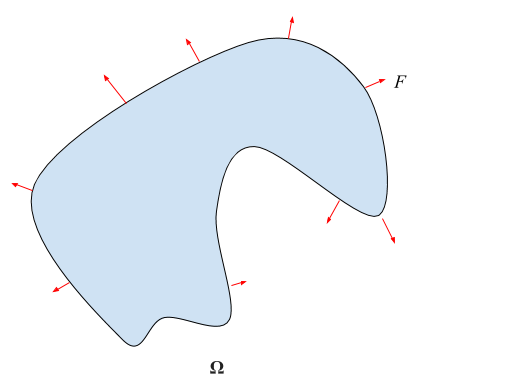
\includegraphics[width=0.5\linewidth]{img/eikonal_vision.png}
  \hfil \caption{распространение кривой со скоростью $F$}
  \label{fig:eikvis}
\end{figure}


Для того, чтобы определить положение волнового фронта в каждый момент
времени, мы можем вычислить время прибытия $T$, когда впервые будет
пересечена точка $(x,y)$.

Если взять одномерный случай, то там мы можем вычислять расстояние как
произведение скорости на время, тогда мы можем записать уравнение для
функции $T$:

\begin{equation*}
  1 = F \frac{dT}{dx}
\end{equation*}

В пространствах более высокой размерности время прибытия $T$ это решение
задачи Дирихле для уравнения эйконала.

\begin{equation}
  \label{eq:eikonal}
  \begin{cases}
    \begin{array}{ll}
      F(x) \| \nabla T(x) \| = 1, x \in \Omega \\
      T(x) = 0, x \in \Gamma
    \end{array}
  \end{cases}
\end{equation}

Здесь $\Omega$ -- это область в $\mathbb{R}^2$, $\Gamma$ -- начальное
состояние кривой, $\nabla$ обозначает градиент, и $\| \cdot \|$ является
евклидовой нормой.

Стоит отметить, что эволюция кривой содержит больше информации чем
время первого прибытия: фронт может проходить через одну и ту же точку
несколько раз. Для иллюстрации рассмотрим распространение
волнового фронта со скоростью $F \equiv 1$, как представлено на
рисунке~\ref{fig:prpgt-eik}

\begin{figure}[h]
  \centering
  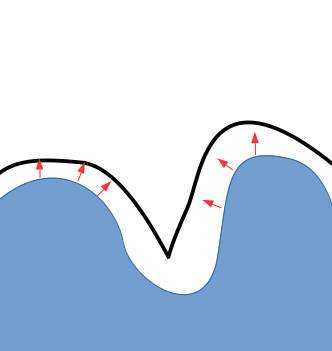
\includegraphics[width=0.3\linewidth]{img/propagate_eikonal.png}
  \hfil \caption{распространение кривой со скоростью $F \equiv 1$}
  \label{fig:prpgt-eik}

\end{figure}

Жирная линия указывает, где будет кривая на следующем шаге.
Предположим, что теперь мы хотим заглянуть дальше. Тогда мы получим
следующую картину на рисунке~\ref{fig:swallow-ex}. Кривая пройдет
сквозь себя, образовав так называемый \textit{ласточкин хвост}. Чем он
плох? Мы в некоторых точках получаем многозначную функцию. В
\cite{S1999}, Sethian сравнивает распространение фронта кривой с
фронтом распространения огня: однажды сожженное второй раз не
сжигается. Следовательно, нам стоит выбрать в каком-то смысле
физически корректное решение как на рисунке~\ref{fig:correct-exmp}

\begin{figure}[h]
  \centering
  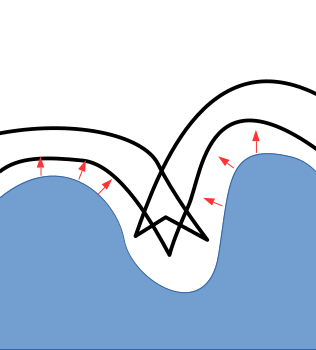
\includegraphics[width=0.3\linewidth]{img/swallow-tail-example.png}
  \hfil \caption{Пример ласточкиного хвоста}
  \label{fig:swallow-ex}

\end{figure}

\begin{figure}[h]
  \centering
  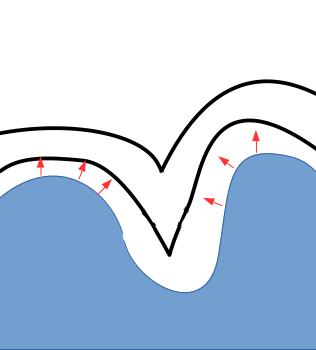
\includegraphics[width=0.3\linewidth]{img/corrct-example.png}
  \hfil \caption{Пример корректного решения}
  \label{fig:correct-exmp}

\end{figure}

Уравнение в задаче~\eqref{eq:eikonal} является частным случаем
\textit{уравнения Гамильтона-Якоби} первого порядка, которое в
стационарном случае приводит к следующей краевой задаче:

\begin{equation}
  \label{eq:hje}
  \begin{cases}
    \begin{array}{ll}
      H(x, \nabla T(x)) = 0,\quad x \in \mathbb{R}^n  \\
      T(x) = 0, \quad  x \in \mathbb{R}^n,
    \end{array}
  \end{cases}
\end{equation}
где гамильтониан $H = H(x,\nabla T(x))$ непрерывная вещественная функция на
$\mathbb{R}^n \times \mathbb{R}^n$ и $T(x) = 0$ -- начальные условия.

Если $H(x,p) = |p| H(x,p/|p|) = |p| F(x)$, тогда мы получаем
обыкновенное уравнение эйконала для изотропного случая
\eqref{eq:eikonal}. Если гамильтониан имеет вид
$H(x,p) = \|p\| F(x, \frac{p}{\|p\|})$, тогда мы имеем анизотропное
уравнение эйконала.

В общем случае это уравнение не имеет классических $C^1$
решений. Задача имеет обобщенные решения, которые
непрерывны и удовлетворяют данному уравнению в частных производных
почти всюду. Использование вязкостных  решений, предложенных в
\cite{V1983,V1984} для задач первого порядка позволяет выбрать одно
``физическое'' решение из множества других. 

\subsection{Вязкостные решения}

В качестве примера рассмотрим следующую задачу

\begin{equation}
  \label{eq:visc_sample}
  \begin{cases}
    \begin{array}{ll}
      |T'(x)| = 1,\quad x \in (-1,1) \\
      T(x) = 0,\quad x = \pm 1
    \end{array}
  \end{cases}
\end{equation}

Здесь мы видим одномерное уравнение эйконала. Общим решением такого
уравнения будет $T(x) = \pm x + c$, но мы не можем выбрать знак $x$ и
константу для того, чтобы удовлетворить граничным условиям. Вместо
этого есть слабое решение, которое удовлетворяет дифференциальному
уравнению почти всюду.

Функция:

\begin{equation*}
  T(x) = 1 - |x|
\end{equation*}

удовлетворяет граничному условию и дифференциальному уравнению почти
всюду, за исключением точки $x = 0$. Это решение дает расстояние до
границы области, но не является единственным. Как показано на
Рисунке~\ref{fig:weak-sol}, существует бесконечно много функций,
удовлетворяющих граничным условиям почти всюду.

\begin{figure}[h]
  \centering
  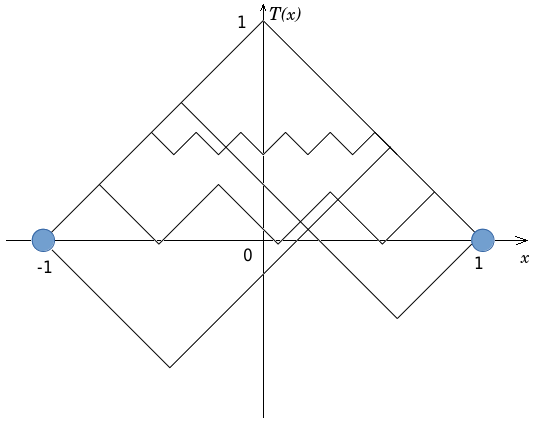
\includegraphics[width=0.5\linewidth]{img/weak-sol.png}
  \hfil \caption{слабые решение $|T'|=1,T(-1)=T(1)=0$}
  \label{fig:weak-sol}
\end{figure}

Если мы добавим к уравнению \eqref{eq:visc_sample} слагаемое,
отвечающее за вязкость, то получим уравнение 2-го порядка для
$T_\epsilon(T)$:

\begin{equation}
  \label{eq:visc_sample_2}
  \begin{cases}
    \begin{array}{ll}
      -\epsilon T''_\epsilon+|T'(x)| = 1,\quad x \in (-1,1) \\
      T_\epsilon(-1) = T_\epsilon(1) = 0.
    \end{array}
  \end{cases}
\end{equation}

Уравнение \eqref{eq:visc_sample_2} имеет единственное решение:

\begin{equation*}
  T_\epsilon(x) = 1 - |x| + \epsilon e^{-1/\epsilon}(1 - e^{(1-|x|)/\epsilon})
\end{equation*}


На рисунке~\ref{fig:viscosity-experiment} изображены решения уравнения
\eqref{eq:visc_sample_2} для $\epsilon =
1/5,1/10,1/20,1/40,1/100$. Для малых $\epsilon$, вязкостный член
сглаживает часть решения $T_\epsilon(x)$. Фактически он сглаживает
углы и делает решение $C^2$ гладким. В этом примере мы выбрали
$\epsilon >0$ для того, чтобы сгладить решение около локальных
максимумов. Выбором $\epsilon <0$ можно получить решения
аппроксимирующие $T(x) = |x| - 1$, которые сглаживают его относительно
локальных минимумов. При стремлении $\epsilon$ к нулю, $T_\epsilon$
сходится к вязкостному решению \eqref{eq:visc_sample}. Подробнее об
этом можно прочесть в работах \cite{V1984,V1983}.


\begin{figure}[h]
  \centering
  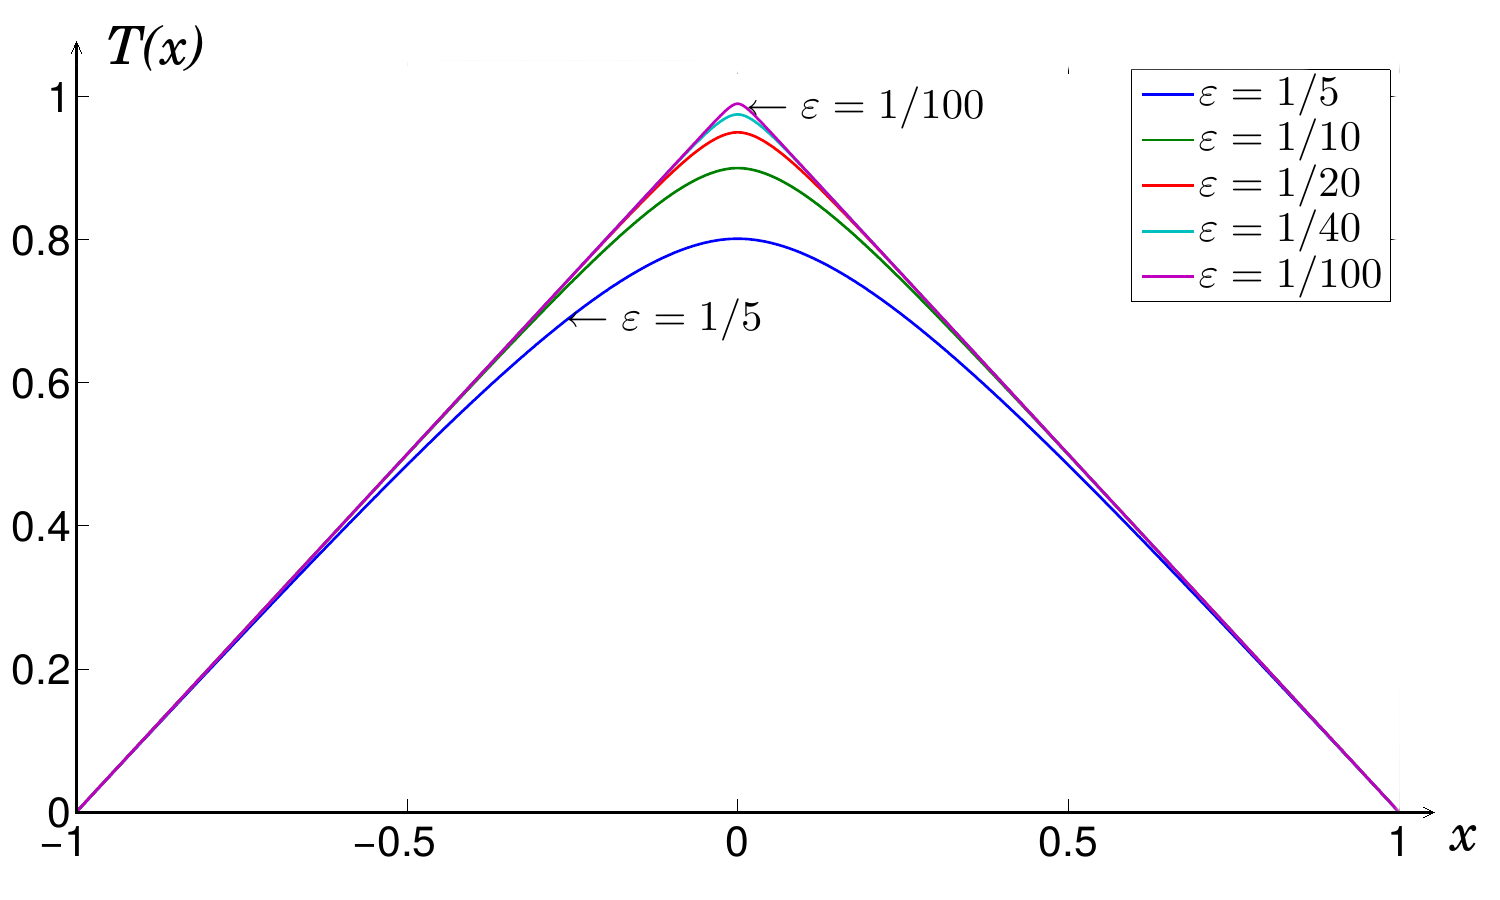
\includegraphics[width=0.6\linewidth]{img/viscosity_example.png}
  \hfil \caption{Решение уравнения \eqref{eq:visc_sample_2} 
	для $\epsilon = 1/5, 1/10, 1/20, 1/40, 1/100$}
  \label{fig:viscosity-experiment}

\end{figure}


% \subsection{Анизотропное уравнение эйконала}

% Предположения, которые выдвигались вначале обзора касались изотропного
% случая, когда на скорость распространения кривой не влияло ее текущее
% местоположение. Мы расширим н\аше уравнение Гамильтона-Якоби


\pagebreak
\section{Численные методы решения}
\label{sec:algrhtms}

Далее мы опишем алгоритмы, использующиеся для численного решения
уравнений эйконала. Первый алгоритм динамически выбирает порядок
обхода узлов, а второй использует несколько фиксированных порядков.
% Один заточен для максимального ускорения работы и,
% как это часто бывает с такими алгоритмами практически неспособен к
% параллелизации, другой же -- наоборот работает несколько медленнее, но
% гораздо проще поддается распараллеливанию.

\subsection{Общая идея методов}
\label{sec:general-idea}

Для всех численных методов  нам необходимо научится решать локальную задачу,
т. е. вычислять значение $T$ в узле по известным значениям в части
соседних узлов. Разберем для начала одномерный случай. Пусть нам дана
следующая краевая задача для уравнения эйконала:

\begin{equation}
  \label{eq:eik_smp}
  \begin{cases}
    \begin{array}{ll}
      \sqrt{(T'(x))^2}=F(x)\\ T(-1) = T(1) = 0.
    \end{array}
  \end{cases}
\end{equation}

Стоит отметить, что в таком виде задача имеет также аналитическое
решение, удовлетворяющее условиям почти всюду

Имеется функция скорости $F(x) > 0$, требуется построить
решение $T(x)$. Мы видим, что решение не уникально (если $t(x)$ решает
задачу, то тогда и $-t(x)$ также ее решает). Будем работать только с
положительными решениями.


Рассмотрим обыкновенное дифференциальное уравнение и разобьем решение
на подзадачи:

\begin{equation*}
  \begin{cases}
      \begin{array}{ll}
        T'(x) = ~F(x), \quad x \ge 0,\\
        T'(x) = -F(x), \quad x \le 0,\\[0.3cm]
        T(-1)= T(1) = 0.
      \end{array}
    \end{cases}
\end{equation*}

Для численной аппроксимации разобьем ось $x$ на набор точек сетки
$x_i=i\Delta x$. Положим $T_i = T(i \Delta x)$ и
$F_i = F(i \Delta x)$, где $\Delta x$ - это шаг дискретизации,
$i = -n, \cdots, n$.

Введем также обозначение для разностных производных первого порядка:

\begin{eqnarray*}
    D^{+x}_iT(x_i) &=& \frac{T_{i+1} - T_{i}}{\Delta x} \\
    D^{-x}_iT(x_i) &=& \frac{T_{i} - T_{i-1}}{\Delta x}
\end{eqnarray*}

Наконец, заменим производные в уравнениях на их разностные аналоги.

\begin{equation}
  \label{eq:discretise}
  \begin{cases}
      T_n = 0,\\
      D^{+x}_iT(x_i) = F_i, \quad i>0 \\
      D^{-x}_iT(x_i)  = F_i, \quad i>0\\
      T_{-n} = 0\\
    \end{cases}
\end{equation}

Отметим, что
\begin{itemize}
\item[ ] $T_{n-1}$ может быть получено из $T_n$
\item[ ] $T_{n-2}$ может быть получено из $T_{n-1}$
\item[ ]  $\cdots$
\item[ ] $T_{1}$ может быть получено из $T_2$
\item[ ] $T_{0}$ может быть получено из $T_{1}$
\item[ ]  $\cdots$
\item[ ] $T_{-n+1}$ может быть получено из $T_{-n}$
\item[ ] $T_{-n+2}$ может быть получено из $T_{-n+1}$
\item[ ]  $\cdots$
\item[ ] $T_{-1}$ может быть получено из $T_{-2}$
\item[ ] $T_{0}$ может быть получено из $T_{-1}$

\end{itemize}

Выше мы построили разностную схему, где вычисляем производные, двигаясь
по направлению распространения границы: каждое следующее уравнение вне
текущей границы получено на основании уже имеющихся решений внутри
нее.

Численно решая уравнение эйконала мы видим, что информация
распространяется как волны с определенной скоростью вдоль направления
градиента. Наш метод дискретизации вычисляет значение времени
достижения точки. Он использует направление, откуда приходит
информация о времени достижения в соседних точках. Если говорить
точнее, то дискретизация уравнений в частных производных использует
конечно-разностную трассировку смещающуюся в направлении знака
градиента.

Для одномерного случая у нас есть только два направления для каждой
точки $i$: правое $(i+1)$ и левое $(i - 1)$. Предположим, что у нас
есть решение в точке $i$, на итерации с номером $n$. Тогда мы имеем
два случая:
\begin{itemize}
\item правое направление: $T_i^{n+1} = T_i^n - \Delta x D^{+x}_iT(x_i)$
\item левое направление: $T_i^{n+1} = T_i^n - \Delta x D^{-x}_iT(x_i)$
\end{itemize}


Подобным образом в точке $(x,y)$ для двумерного случая мы можем
определить эти обозначения для величины $T$. Тем самым мы задаем
регулярную двумерную сетку дискретизации, тогда для точек $(x,y)$, с
разбиением $(x_i,y_i) = (i\Delta_x,j \Delta_y)$ (их еще называют
узлами сетки) и $T_{ij} = T(x_i,y_i)$ мы получим:

\begin{equation}
  \begin{aligned}
  \label{eq:discrete-defines}
    D^{-x}_{i,j}T(x,y) &=& \frac{T_{i,j} - T_{i-1,j}}{\Delta_x}  \\
    D^{+x}_{i,j}T(x,y) &=& \frac{T_{i+1,j} - T_{i,j}}{\Delta_x}  \\
    D^{-y}_{i,j}T(x,y) &=& \frac{T_{i,j} - T_{i,j-1}}{\Delta_y}  \\
    D^{+y}_{i,j}T(x,y) &=& \frac{T_{i,j} - T_{i,j+1}}{\Delta_y}
    \end{aligned}
\end{equation}

\begin{itemize}
\item $D^{+x}$ вычисляет новое значение в узле сетки $(i,j)$, используя
  информацию из $i$ и $i+1$, таким образом информация для решения
  распространяется справа налево.

\item $D^{-x}$ вычисляет новое значение в узле сетки $(i,j)$, используя
  информацию из $i$ и $i-1$, таким образом информация для решения
  распространяется слева направо.
\item $D^{+y}$ вычисляет новое значение в узле сетки $(i,j)$, используя
  информацию из $j$ и $j+1$, таким образом информация для решения
  распространяется сверху вниз.

\item $D^{-y}$ вычисляет новое значение в узле сетки $(i,j)$, используя
  информацию из $j$ и $j-1$, таким образом информация для решения
  распространяется снизу вверх.

\item 
\end{itemize}

% добавить по двум направлениям 

Для двумерного случая с использованием двух направлений одновременно
разностные схемы действуют вдоль направления градиента. На
рисунке~\ref{fig:upwind-schema} иллюстрируются две возможных
ситуации. В первом случае распространение информации идет из третьего
квадранта, В другом случае -- из второго
\begin{figure}[H]
  \centering
  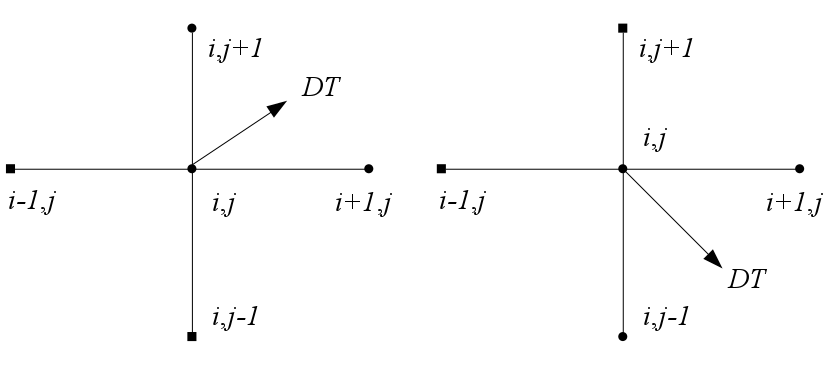
\includegraphics[width=\linewidth]{img/upwind-schema.png}
  \hfil \caption{Пример разных направлений распространения}
  \label{fig:upwind-schema}

\end{figure}

Крэндалл и Лайонс в \cite{V1983} доказали, что последовательные
монотонные схемы сходятся к корректному вязкостному решению. Поэтому
мы можем развивать идеи дальше и применить сказанное выше к уравнениям
эйконала. Существует несколько различных схем приближения. Мы
воспользуемся схемой Годунова \cite{G1956,F2002}:

\begin{equation}
  \label{eq:godunov-schema}
  % \begin{cases}
  %   \begin{matrix}
       \max (D^{-x}_{ij}T, -D^{x}_{ij},0)^2 + 
	  \max (D^{-y}_{ij}T, -D^{y}_{ij},0)^2
  %   \end{matrix}
  % \end{cases}
  = \frac{1}{F_{ij}^2}
\end{equation}

% Рассмотрим, как будет работать схема Годунова на простом примере:
% $\Delta x = 1$ и $F(x) = 1, 1 < i < n$ и покажем, что она выделяет
% только вогнутые решения:


% Как мы можем решить уравнение \eqref{eq:godunov-schema}? Предположим,
% что у нас есть сетка. Рассмотрим один ее узел и 4 ближайших ее соседа
% см. рисунок~\ref{fig:rec-grid-node}

% \begin{figure}[ht]
%   \centering
%   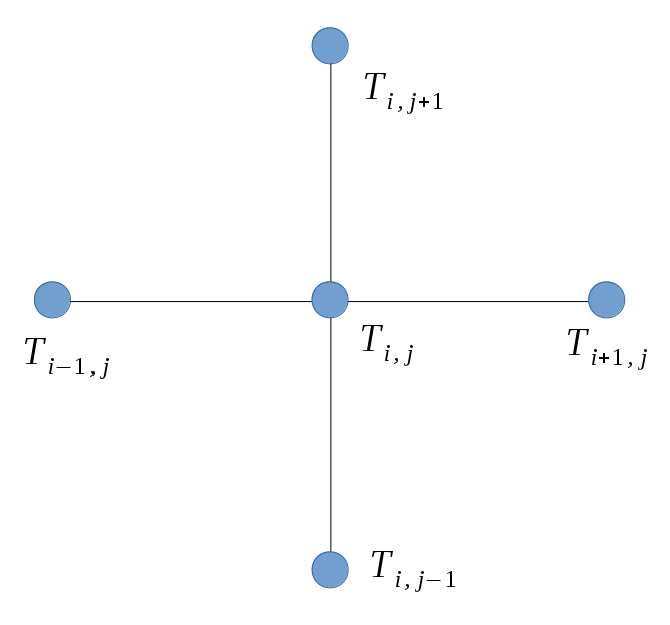
\includegraphics[width=0.5\linewidth]{img/rec-grid-node.png}
%   \hfil \caption{Узлы сетки}
%   \label{fig:rec-grid-node}

% \end{figure}

% Нам нужно выяснить значение $T_{i,j}$. Если исходить из оговоренных в
% постановке задачи условий, хотя бы одна из соседних точек имеет
% числовое значение,

Далее мы подставляем наши разностные производные
\eqref{eq:discrete-defines} в схему Годунова \eqref{eq:godunov-schema}
и получим

\begin{equation}
  \begin{aligned}
  \label{eq:replaced}
    T &= T_{i,j}\\
    T_{x}&= \min(T_{i-1,j},T_{i+1,j})\\
    T_{y}&= \min(T_{i,j-1},T_{i,j-1})
      \end{aligned}
\end{equation}

Уравнение эйконала может быть переписано для дискретного двумерного
случая на прямоугольной сетке следующим образом:
% \begin{equation*}
%   \sqrt{\max \left( \frac {T-T_{x}}{\Delta_x},0 \right)^2+  \max \left( \frac
%   {T-T_{y}}{\Delta_y},0\right)^2} = \frac{1}{F_{i,j}}
% \end{equation*}
% Или эквивалентно, можем записать:

\begin{equation}
  \label{eq:discrete-eikonal}
  \max \left( \frac {T-T_{x}}{\Delta_x},0 \right)^2+  \max \left( \frac
      {T-T_{y}}{\Delta_y},0\right)^2 = \frac{1}{F_{i,j}^2}
\end{equation}

Поскольку предполагается, что скорость распространения фронта
положительная $(F>0)$, поэтому $T$ будет больше чем $T_x$ и $T_y$ когда фронт
еще не посещал точку $(i,j)$. Следовательно уравнение
\eqref{eq:discrete-eikonal} можно безболезненно переписать еще раз:

\begin{equation}
  \label{eq:discrete-eikonal-2}
  \left( \frac {T-T_{x}}{\Delta_x} \right)^2+
  \left( \frac {T-T_{y}}{\Delta_y} \right)^2 = \frac{1}{F_{i,j}^2}
\end{equation}

Уравнение \eqref{eq:discrete-eikonal-2} обычное квадратное уравнение
вида $aT^2+bT+c=0$ где:

\begin{equation}
  \begin{aligned}
  \label{eq:replaced}
    a &= \Delta_2 x + \Delta^2 y\\[0.4cm]
    b &= -2(\Delta^2y T_{x}+\Delta^2x T_{y})\\
    c &= \Delta^2 y T_{y}^2 + \Delta^2 x T_{x}^2 - \frac{\Delta^2 x
      \Delta^2 y}{F_{ij}^2}
    \end{aligned}
\end{equation}

В качестве решения в текущем узле мы берем меньшее решение квадратного
уравнения. В случае, когда решить его невозможно, мы используем одно
из двух направлений.

\subsection{Fast marching method на прямоугольной сетке}
\label{sec:fast-marching-method}

Fast marching method (FMM) \cite{S1999} является наиболее
распространенным способом численного решения уравнения эйконала. По своей
структуре он напоминает алгоритм Дейкстры. Главное отличие этого
алгоритма в том, что FMM иногда вычисляет значение по двум соседним
точкам, а Дейкстра всегда по одной соседней точке. 

Следовательно, для алгоритма Дейкстры, значение каждого узла $x_i$ зависит только от
родительского узла ${x_j}$, следуя принципу оптимальности Беллмана.

\begin{equation*}
  T_i = \min_{x_i\in \mathcal{N}} (c_{ij} + T_j)
\end{equation*}

Другими словами узел $x_i$ присоединенный к $x_j$ в его
окрестности $\mathcal{N}(x_i)$ минимизирует (или
максимизирует) значение функции (в этом случае $T_i$)состоящей в
значении функции $T_j$ плюс добавленная стоимость движения из $x_j$ в
$x_i$, представленной как $c_{ij}$.

FMM также следует принципу оптимальности Беллмана, но значения для
каждого узла получается из дискретизации уравнения эйконала,
описанного выше. Эта дискретизация учитывает при подсчитывании
значения всех соседей, поэтому FMM может вычислять, в частности,
евклидовы расстояния.

Алгоритм помечает ячейки тремя различными метками:
\begin{enumerate}
\item Изведанная ($\proc{Known}$): значение в этой ячейке не подлежит более
  пересмотру,
\item Неизведанная ($\proc{Unknown}$): ячейка, значение в которой еще не
  получено,
\item Пробная ($\proc{Trial}$): лежит на границе между Изведанными
  и Неизведанными ячейками, значения функции в этих ячейках
  уже известны, но не определены.
\end{enumerate}

Процедура, описанная ниже, инициализирует все точки в сетке в состояние
Неизведанное c бесконечным временем достижения. Стартовые
точки устанавливаются в $0$ и считаются Изведанными. Далее основной
цикл FMM начинает выбирать узлы с наименьшим временем прибытия из
Пробных узлов. Для всех соседей этого узла, не являющихся
Изведанными, решается уравнение эйконала и получается новое
значение времени прибытия. Если оно оказалось меньше чем текущее
значение, то оно заменяет старое. Если соседняя точка была
Неизведанной, то она становится пробной. Наконец, выбранная
точка становится Изведанной, и начинается новая итерация
алгоритма, пока у нас существуют Пробные точки. Полученная
сетка, где в каждом узле наименьшее возможное время прибытия в нее
является результатом работы алгоритма.

FMM нуждается в представлении множества Пробных узлов, для
выполнения над ними следующих операций:
\begin{itemize}
\item Вставка : вставить новый элемент в множество
\item Изменение: изменить порядок элемента, значение которого было
  улучшено
\item Вершина: вернуть элемент с наименьшим значениями
\item Удаление: удалить элемент с наименьшим значением 
\end{itemize}
В реализации нашего алгоритма это наиболее критичный аспект для
увеличения скорости его работы. Наиболее эффективный способ --
использовать неубывающую пирамиду \cite{K2017}.В русскоязычной
литературе существует два термина, которые сводятся к одному в
английском языке --- это пирамида и куча. В переводе \cite{K2017} есть
комментарии по этому поводу. Вслед за переводчиками будем использовать
понятие ``пирамида''. Пирамидой называют упорядоченное дерево, в
котором каждый родитель упорядочивается относительно своих потомков. В
неубывающей пирамиде элемент с минимальным значением находится в корне
дерева, а все потомки имеют большее числовое значение. Это выполняется
для каждого элемента пирамиды.

Обычно пирамиду реализуют через бинарную пирамиду. Тем не менее,
Фибоначчиева пирамида \cite{F1987} имеет лучшее время действия для
изменения и добавления элементов, но она имеет дополнительные
вычислительные расходы по отношению к другим реализациям пирамид. Для
относительно маленьких сеток, где Пробных элементов не так много
бинарная куча работает лучше. Таблица~\ref{tab:perf} отражает
сложность по времени для этих структур (очередь c приоритетом будет
рассмотрена далее). Стоит отметить, что $n$ здесь --- это количество
узлов на сетке, которые нам предстоит посчитать. В худшем случае у нас
все узлы окажутся в пирамиде.

\begin{table}
  \centering
  \caption{Сводная информация об усредненных вычислительных
    сложностях по времени для пирамид (n -- количество элементов в
    пирамиде)}
  \label{tab:perf}
  \begin{tabular}{|*{5}{c|}}
    \hline
Реализация & Вставка & Изменение & Вершина & Удаление\\[0.3cm]\hline
Фиббоначиева пирамида & $O(1)$ & $O(1)$&$O(1)$&$O(\log n$) \\\hline
Двоичная пирамида & $O(\log n)$ & $O(\log n)$&$O(1)$&$O(\log n$) \\\hline
Очередь приоритетов & $O(\log n)$ & -- &$O(1)$&$O(\log n)$ \\\hline
  \end{tabular}
\end{table}

В каждой итерации вершина пирамиды Пробных точек достигается за
константу $O(1)$, эйконал решается для не более чем для $2^N$
соседей ($O(1)$ для данного $N$), эти точки вставляются или
изменяются (в худшем случае за $O(\log n)$) И наконец, вершина
удаляется за $O(\log n)$. Следовательно каждая итерация цикла
работает не хуже чем за $O(\log n)$. Поскольку цикл выполнится не
более чем $n$ раз, мы сложность FMM ограничивается сверху $O(n \log n)$

Существует некоторое упрощение алгоритма FMM в котором мы не изменяем
значения пробных ячеек, а храним их все. В том числе и разных
типов. Сделать такое нам позволяет очередь приоритетов. Каждый раз,
когда мы получаем новое значение, мы вставляем его в нашу очередь.

Этот метод позволяет нам заменить операцию изменения на операцию
вставки, кроме того, как было указано выше - алгоритм имеет такую же
временную сложность как и другие: $O(n\log n)$

\subsection{Fast sweeping method на прямоугольной сетке}
\label{sec:fast-sweeping-method}

Fast sweeping method (далее FSM) -- итеративный метод, основная идея
которого -- последовательно ``замести'' сетку в определенных
направлениях. C точки зрения системы разностных уравнений FSM
выполняет итерации Гаусса-Зейделя в чередующихся направлениях. Эти
направления выбираются так, чтобы все возможные характеристические
кривые решения эйконала делились на возможные квадранты.


Двумерная сетка имеет 4 возможных направления для итерации
Гаусса-Зейделя: различные попарные комбинации вдоль $x$ и $y$ вперед и
назад смотри рисунок~\ref{fig:fsm-sweeps}


\begin{figure}[H]
  \centering
  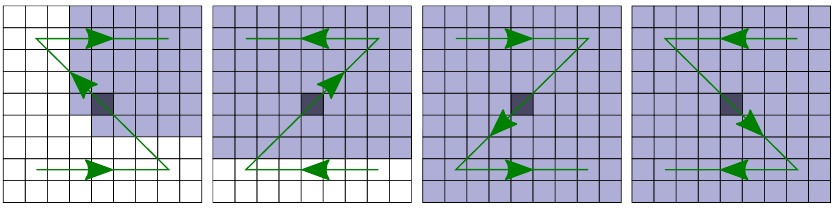
\includegraphics[width=\linewidth]{img/fsm-sweeps.png}
  \hfil \caption{Направления выметаний на двумерной сетке, указаны
    стрелками. Самая темная стрелка -- это стартовая точка,
    затемненные -- проанализированные текущим выметанием}
  \label{fig:fsm-sweeps}

\end{figure}

FSM --- простой алгоритм, выполняющий выметания до тех пор, пока
значение не будет утверждено. В каждом выметании эйконал решается для
каждой ячейки, и если значение оказалось меньше текущего, то старое
заменяется на новое. Для порядка выметаний используется массив
$\proc{SweepDirs}$, содержащий в себе значения $1$ или $-1$,
подразумевающие направления вперед и назад, по текущему направлению,
мы инициализируем массив единицами, а сетку -- аналогично тому, как
это сделано в алгоритме FMM. Каждую итерацию мы обновляем значения
одного из элементов $\proc{SweepDirs}$, так чтобы пробегались все
возможные значения, для прохождения нужных выметаний. Наконец сам
алгоритм FSM выполняет итерацию Гаусса-Зейделя следуя направлениям
заданным $\proc{SweepDirs}$.

Этот метод проходит сетку до тех пор, пока для каждого $T_i$ не утвердится
его значение, что означает, что на текущем проходе все $T_i$ не изменились.
Для ка каждой ячейки стоимость вычисления уравнения Эйконала -- $O(1)$.
Поскольку существует $n$ узлов, общая сложность FSM $O(n)$ однако, стоит
отметить, что константы этого выражения сильно зависят от функции скорости
$F(x)$. В случае пустого поля с постоянным $F(x)$, нужно только $4$
выметания, так как характеристиками в таком случае являются прямые линии
однако для более сложных сеток с препятствиями (или более сложных функций
скорости), где характеристики часто меняют свое направление, нам может
понадобится гораздо большее число выметаний, и поэтому FSM - будет работать
дольше.

\subsection{Fast sweeping method на нерегулярной сетке}
\label{sec:unstructured-mesh}

Теперь мы хотим попробовать изменить нашу квадратную сетку на
нерегулярную, для большей свободы определения значений. Для этого
возьмем за основу не прямоугольник, как это было раньше, а треугольник
--- фигура, которой гораздо проще приближаются различные
многоугольники. В частности регулярная прямоугольная сетка (тоже легко
моделируется треугольной сеткой)

Сложность работы с треугольной сеткой в том, что мы не можем просто
разбить на несколько случаев варианты расположений соседних точек,
теперь соседних точек может оказаться как больше так и меньше $4$, и
их положение не определено регулярной структурой. Поэтому, нам нужно
по другому считать локальное решение уравнения эйконала.

Мы все также исследуем уравнение \eqref{eq:eikonal}, только теперь мы
предположим, что $\Omega$ разбита на непересекающиеся, непустые
треугольники $\mathcal{T}$ с диаметром $h_{\mathcal{T}}$, так чтобы
$\Omega = \bigcup_{\mathcal{T}\in \mathcal{T}_h}\mathcal{T}$ Мы
полагаем, что $\mathcal{T}_h$ удовлетворяет следующим условиям.
\begin{itemize}
\item Не более чем $\mu$ треугольников имеют общую вершину; 
\item $h = \sup_{\mathcal{T} \in \mathcal{T}_h}\mathcal{T}$<1;
\item Существует такая константа $\omega_0$, независящая от $h$ такая,
  что если $\rho_{\mathcal{T}}$ диаметр наибольшего шара
  $B \subset \mathcal{T}$, тогда для всех
  $\mathcal{T} \in \mathcal{T}_h,\ h_{\mathcal{T}} \le \omega_0
  \rho_{\mathcal{T}}$
\end{itemize}

Для данного треугольника $\vartriangle ABC$ мы обозначим за $\angle A =
\beta $, $\angle B = \alpha$ и $\angle C~=~\gamma$, а за $\overline{AB} =
c,\ \overline{AC} =b,\ \overline{BC} =a$ длины соответствующих сторон
$AB$, $AC$, и $BC$ соответственно.

Мы считаем, что треугольной сеткой мы задаем кусочно-линейную
аппроксимацию. Фронт распространения кривой обновляет значение времени
прибытия в узле $C$, исходя из значений $T_A$ и $T_B$, для точек $A$ и
$B$ соответственно. Мы полагаем, что луч исходящий из точки $C$ и
ортогональный фронту должен проходить внутри $\vartriangle ABC$

Отметим, что направление изотропного распространение волны совпадает с
направлением градиента поля решения.

Сначала предположим, что $\vartriangle ABC$ остроугоьный. Чтобы
построить схему первого порядка, мы определяем плоский волновой фронт
по известным значениям $T_A$ и $T_B$. Предположим, что угол $\theta$
между фронтом распространения и и ребром $AB$.

Без потери общности мы также предполагаем, что $T_B \ge T_A$. Если
$T_C$ определяется через $T_A$ и $T_B$, тогда по принципу Гюгенса
фронт волны должен пройти сначала через вершину $A$, затем через
вершину $B$, и наконец $C$. Чтобы это гарантировать, надо чтобы
выполнялись следующие условия:
\begin{itemize}
\item $|T_B-T_A| / f_C \le \overline{AB} = c$ т.е., это означает
  возможность фронта от $A$ до $B$ с данной скоростью, где $f_c$ - это
  обратное значение скорости в точке $F(C)$;
\item $\theta \le \alpha$ это означает, что фронт пройдет через $B$
  раньше чем через $A$
\item $\theta + \beta < \frac{\pi}{2}$ в противном случае нарушается
  условие причинности потому, что ортогональная линия от $C$ к фронту
  проходит вне треугольника. Смотри рисунок~\ref{fig:triangle-front}
\end{itemize}

\begin{figure}[H]
  \centering
  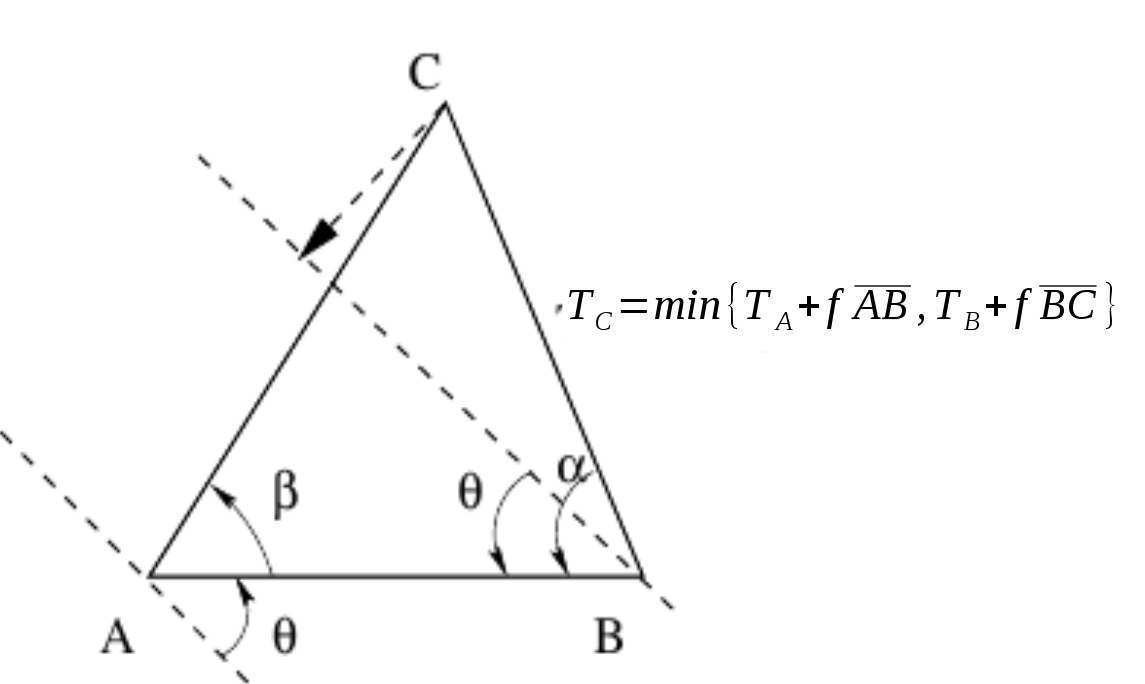
\includegraphics[width=0.7\linewidth]{img/triangle-front.png}
  \hfil \caption{Изменение значения в вершине С, c нарушенным условием
  причинности}
  \label{fig:triangle-front}

\end{figure}

Если все $n$ треугольников
$\mathcal{T}_1,\mathcal{T}_2,...,\mathcal{T}_n$ вокруг $C$
остроугольные, фронт волны может быть захвачен одним из треугольников.

Из всего выше сказанного мы можем получить следующий алгоритм для
нахождения локального решения. Общая его идея состоит в
следующем. Если нарушаются условия для того, чтобы считать
распространение фронта через точки $A$ и $B$, тогда фронт идет от
одной из вершин. В таком случае выбираем вершину из которой фронт
пришел быстрее.

\begin{enumerate}
\item если $|T_B-T_A| \le c f_C$, тогда
  \begin{equation*}
    \theta = arcsin \left(\frac{|T_B-T_A|}{c f_C}\right);
  \end{equation*}
  \begin{enumerate}
  \item если $\max (0,\alpha - \frac{\pi}{2}) \le \theta \le
    \frac{\pi}{2} - \beta$ или $\alpha - \frac{\pi}{2} \le \theta \le
    \min(0, \frac{\pi}{2} - \beta)$, тогда
    \begin{equation*}
      \begin{aligned}{c}
        h = \overline{CP} = a \sin(\alpha - \theta); H =
        \overline{CQ}=
        b \sin (\beta + \theta);\\
        T_C = \min\{T_C,0.5(h f_C + T_B)+0.5(H f_C + T_A)\};
      \end{aligned}
    \end{equation*}
  \item иначе
    \begin{equation*}
      T_C = \min\{T_C,T_A+b f_C, T_B + a f_C\};
    \end{equation*}
  \end{enumerate}
\item иначе
  \begin{equation*}
    T_C = \min{T_C,T_A+b f_C, T_B + a f_C};
  \end{equation*}

\end{enumerate}

Теперь для того, чтобы определить значение $T_C$ мы применим эту
процедуру для каждого пары точек соседних с $T_C$ и установим
наименьшее из полученных значений как решение в этой точке

Связываясь с треугольной сеткой мы получаем еще одну задачу - как в
рамках алгоритма FSM нам проводить процедуру выметания? Теперь у нас
нет жесткого порядка, по которому мы можем пройтись, однако мы его
можем установить. Для этого нам необходимо выделить несколько точек на
плоскости и относительно каждой  отсортировать остальные точки в порядке
удаления от нее и проводить выметания по таким направлениям в сторону
возрастания и в сторону убывания. В работе \cite{FS2007} также
утверждается, что для двумерного случая достаточно всего 3-х
точек. Таким образом будет 6 направлений выметаний.

Условия остановки алгоритма остались те же самые, что и в обыкновенном
FSM. В этом алгоритме добавляется другой критичный параметр для
вычислительной трудности: сортировка всех точек. Здесь уже давно
получены результаты вплоть до сортировки за линейное время набора
целочисленных точек \cite{K2017}. Проблема же с количеством выметаний
ровно та же, что и в классическом FSM

Отдельной задачей в этом методе является построение из разрозненных
точек системы треугольников. Причем таких, чтобы как можно больше
углов у них были острыми. Эта задача триангуляции Делоне \cite{T2002}

% рисунок с несколькими опорными точками и фронтом пробегания по
% остальным точкам

% \subsubsection{Триангуляция}
% \label{sec:triangulate}


\subsection{Fast sweeping method для анизотропного случая}

Теперь поразмыслим - что будет если мы для скорости $F$ предположим
наличие не только направления по нормали от фронта распространения
волны. Мы получаем в таком случае анизотропное распространение, где
направление фронта не так просто вычислить. Мы уже не можем
представить наше уравнение как в задаче \eqref{eq:eikonal}, поэтому
берем более общий случай - уравнение Гамильтона-Якоби и,
соответственно, задачу \eqref{eq:hje}

Если мы возьмем треугольную сетку, как это было сделано выше, то
направление фронта получается из любой точки на основании $AB$,
треугольника $ABC$.

Мы вводим треугольную сетку также, как это было сделано в
\ref{sec:unstructured-mesh}, только теперь формулы вычисления
локального решения будут другие.

Если $T_A$ и $T_B$ используются для обновления вершины $T_C$, должен
быть луч, исходящий из отрезка $AB$, к точке $C$, которую мы назовем
$F(s)$. Эта точка расположена между $A$ и $B$, а $s$ параметризует
$AB$ таким образом, что $F(0)=A$ и $F(1) = B$.

Пользуясь принципом Ферма, время прибытия в $C$ получится путем
минимизирования по $s$ следующего функционала:

\begin{equation}
  \label{eq:2}
  T_C(s) = sT_B + (1-s)T_A + \frac{d(s)}{v_g(C)},
\end{equation}

где $d(s) = \overline{CF(s)} = \sqrt(b^2+c^2s^2-2bcs \cos \beta)$, а
параметр $v_g$ - так называемый вектор группы скоростей, который
указывает в направлении действия луча $CF(s)$

\begin{equation}
  \label{eq:3}
  v_g(x,p) = \left| \frac{dx}{dt} \right| = \left| \nabla_p H  \right|
\end{equation}


\subsection{Вопросы реализации}
\label{sec:programming}

Для реализации всего вышеперечисленного было решено воспользоваться
языком программирования C \cite{C2017}, который считается тонким
связующим уровнем с системой \cite{AP2016}, что позволяет очень точно
контролировать ресурсы компьютера. Поскольку предполагается большой
объем вычислений с различными структурами данных, которые не потянет
ни один скриптовый язык. В работах \cite{AVS2016, AV2015_1, AV2015_2}
как раз использовался язык python. Даже с окружение Scientiffic Python,
модули которого реализованы на компилируемых языках C и Fortran мы не
могли добиться нужного быстродействия. Поскольку здесь алгоритмам
требуется изменять саму сетку, а не только быстро вычислять значения,
т.е.нам приходится постоянно подниматься на уровень python из
библиотеки и выполнять медленные операции передачи информации на
другой модуль SciPy и так каждую итерацию алгоритма. Поэтому было
решено взять язык C.

Вначале был реализован метод FMM. Причем на первом этапе вычисление
$F$ включалось внутрь самой программы, что требовало ее
перекомпиляции каждый раз для смены формулы.

Так как мы реализовывали FMM для прямоугольной сетки, то мы можем
воспользоваться скоростью доступа и изменения значений от
массивов. Поэтому сетка реализована в виде двумерного массива, но
кроме того, нам нужна отдельно очередь приоритетов, как это было
сказано в \ref{sec:fast-marching-method}, для которой мы использована
ее реализация в библиотеке Glib. Для каждого узла мы храним i,j ---
индексы, текущей точки

Основную вычислительную нагрузку берет на себя функция
process\_neighbour (см. Листинг 1), который вызывается для каждого соседа той точки,
значение в которой сейчас наблюдается (было получено из очереди
приоритетов) Листинг 2.

\vspace{1em}
Листинг 1 --- вычисление значения в узле 
\normalsize
\begin{verbatim} 
void process_neighbour(int i, int j)
{
  Node node = {i,j};
  if (!is_internal(node) || 
      !gsl_matrix_get(K, i, j)) 
    return;
  double lT = gsl_matrix_get(T, i - 1, j);
  double rT = gsl_matrix_get(T, i + 1, j);
  double uT = gsl_matrix_get(T, i, j - 1);
  double dT = gsl_matrix_get(T, i, j + 1);

  double mini = lT < rT ? lT : rT;
  double minj = uT < dT ? uT : rT;

  double time;

  if (finite(mini) && isinf(minj))
    time = mini + x_step/speed(node);
  else if (finite(minj) && isinf(mini))
    time = minj + y_step/speed(node);
  else if (finite(mini) && finite(minj)){
    double a = 1/(x_step*x_step) + 
               1/(y_step*y_step);
    double b = -2 * (mini/pow(x_step, 2) +
                     minj/pow(y_step,2));
    double c = pow(mini/x_step, 2) + 
               pow(minj/y_step, 2) - 
               1.0/speed(node);
    double x1,x2;
    int croots = gsl_poly_solve_quadratic(a,b,c, 
                                        &x1, &x2);
    if (croots == 0)
      time = INFINITY;
    else if (croots == 1)
      time = x1;
    else if (croots == 2)
      time = x2;
  }
  if (time < gsl_matrix_get(T, i, j)){
    gsl_matrix_set(T, i, j, time);
    g_queue_insert_sorted(active_nodes,
                          make_node(i,j),
                      (GCompareDataFunc)cmp,NULL);
  }
}
\end{verbatim}
\large


\vspace{1em}
Листинг 2 --- выбор точки и обработка ее соседей
\normalsize
\begin{verbatim} 
void process_neighbour(int i, int j)
{
  while (!g_queue_is_empty(active_nodes)) {
    Node* node = g_queue_pop_head(active_nodes);
    gsl_matrix_set(K, node->i, node->j,0);
    process_neighbour(node->i - 1, node->j);
    process_neighbour(node->i + 1, node->j);
    process_neighbour(node->i, node->j - 1);
    process_neighbour(node->i, node->j + 1);
  }

}
\end{verbatim}
\large



Далее был реализован метод FSM, его особенность в том, что ему
достаточно только структуры сетки. Процесс вычисления направления
выметания реализовывался следующей функцией Листинг 2.3

\vspace{1em}
Листинг 3 --- инициализация направлений
\normalsize
\begin{verbatim} 
void get_sweep_dirs()
{
        for(int i = 0; i < 2; i++) {
                sweep_dirs[i] += 2;
                if (sweep_dirs[i] <= 1)
                        break;
                else
                        sweep_dirs[i] = -1;
        }
}

\end{verbatim}
\large

Далее происходил процесс выметания в направлении, указанном массивом
sweep\_dirs. Там необходимо переключать направление работы цикла для
верного вычисления координат. Все это вычисляется функций sweep
Листинг 4


\vspace{1em}
Листинг 4 --- процесс выметания
\normalsize
\begin{verbatim} 
bool sweep(int n, int* pos)
{
  bool stop = true;
  if (n > 0){
    for (int i = 0; i < F->size2; i++){
      if (sweep_dirs[n] == 1)
        pos[n] = i;
      else
        pos[n] = F->size2 - i - 1;
      stop = sweep(n - 1, pos);
    }
  }
  else
    for (int i = 0; i < F->size1; i++){
      if (sweep_dirs[n] == 1)
        pos[n] = i;
      else
        pos[n] = F->size1 - i - 1;

      double time = process_neighbour(pos[0],pos[1]);

      if (time < gsl_matrix_get(T, pos[0], pos[1])){
               
        gsl_matrix_set(T, pos[0], pos[1], time);
        stop = false;
      } 

    }
  return stop;

}
\end{verbatim}
\large

В предыдущих случаях нам не было нужды организовывать проект,
поскольку все, что нам было нужно легко помещалось в один файл. Для
организации же неструктурированной сетки нам пришлось отказаться от
простой и наглядной (на первый взгляд) идеи массива в качестве основы
для сетки. Теперь вся она представляет собой граф, где каждый узел
хранит в себе необходимые значения скорости в текущей точке, координат
и значения искомой функции.

Граф был реализован на основании списках смежности смотри Листинг 5 и
Листинг 6, поскольку у каждого узла сетки лишь малое количество
соседей по сравнению с общим их числом.

\vspace{1em}
Листинг 5 --- Заголовочный файл для графа
\normalsize
\begin{verbatim}
#ifndef GRAPH_H
#define GRAPH_H 1

#include <stdbool.h>

struct link
{
        struct vertex* vertex;
        struct link* next;
};

struct vertex
{
        int id;
        int cnt_dims;
        double *coords;
        double fx;
        double ux;
};

struct graph
{
        int cnt_vertices;
        int cnt_edges;
        struct vertex* vertices;
        struct link** adj;
};

struct graph* make_graph(int cnt_vertices, 
                         int cnt_dims,
                         double** coords, 
                         double* values,
                         double* init_u);
void graph_connect(struct graph*, 
                   int, int);
bool graph_is_connected(struct graph*, 
                        int, int);
struct link* graph_get_neighbours(
                        struct graph* g, 
                        int id);

#endif // GRAPH_H

\end{verbatim}
\large


\vspace{1em}
Листинг 6 --- Реализация графа
\normalsize
\begin{verbatim}

#include <stdlib.h>
#include <stdbool.h>
#include <math.h>

#include "graph.h"

void fill_vertex(struct vertex* v, 
                 int cnt_dims, 
                 double* coords, 
                 double fx, 
                 double ux)
{
  v->cnt_dims = cnt_dims;
  v->coords = coords;
  v->fx = fx;
  v->ux = ux;
}

struct link *new_link(struct vertex* vertex, 
                      struct link* next)
{
  struct link* x = malloc(sizeof(struct link));
  x->vertex = vertex;
  x->next = next;
  return x;

}

struct graph* make_graph(int cnt_vertices, 
                         int cnt_dims ,
                         double* coords[],
                         double* values,
                         double* init_u)
{
  struct graph* g = malloc(sizeof (struct graph));
  g->cnt_vertices = cnt_vertices;
  g->cnt_edges = 0;
  g->vertices = 
    malloc(sizeof(struct vertex) * cnt_vertices);
  for (int v = 0; v < cnt_vertices; v++) {
    fill_vertex(&g->vertices[v],
                 cnt_dims,coords[v],
                 values[v],init_u[v]);
    g->vertices[v].id = v;
  }
  g->adj = 
    malloc(sizeof(struct link) * cnt_vertices);
  for (int v = 0; v < cnt_vertices; v++) {
    g->adj[v] = NULL;
  }
  return g;
}

void graph_connect(struct graph* g, 
                   int id1, int id2)
{
  struct vertex* v1 = &g->vertices[id1];
  struct vertex* v2 = &g->vertices[id2];
  g->adj[id1] = new_link(v2, g->adj[id1]);
  g->adj[id2] = new_link(v1, g->adj[id2]);
  g->cnt_edges++;
}

bool graph_is_connected(struct graph* g, 
                        int id1, int id2)
{
  for(struct link* t =g->adj[id1]; 
         t != NULL; t = t->next)
    if (t->vertex->id == id2) return true;
  return false;
}

struct link* graph_get_neighbours(
              struct graph *g, int id)
{
  return g->adj[id];
}

\end{verbatim}
\large

Кроме того в соответствии с формулами \ref{sec:unstructured-mesh} мы
получаем другую функцию для вычисления локального решения мы вычисляем
необходимые параметры треугольника функцией set\_triangle, а функцией
solve\_ndims находим решение в точке.

\vspace{1em}
Листинг 2.7 --- Реализация решения на треугольной сетке
\normalsize
\begin{verbatim}
void set_triangle(struct vertex* v, 
                  struct vertex* v1, 
                  struct vertex* v2,
                  double* a, 
                  double* b, 
                  double* c,
                  double *al, 
                  double* bt)
{
  double b2c = 0;
  double a2c = 0;
  *a=*b=*c=0;
  for (int i = 0; i < v->cnt_dims; i++){
    *a += (v->coords[i] - v2->coords[i])*
          (v->coords[i] - v2->coords[i]);
    *b += (v->coords[i] - v1->coords[i])*
          (v->coords[i] - v1->coords[i]);
    *c += (v1->coords[i]- v2->coords[i])*
          (v1->coords[i]- v2->coords[i]);
    b2c+= (v->coords[i] - v2->coords[i])*
          (v1->coords[i]- v2->coords[i]);
    a2c+= (v->coords[i] - v1->coords[i])*
          (v2->coords[i]- v1->coords[i]);
  }
  *a = sqrt(*a);
  *b = sqrt(*b);
  *c = sqrt(*c);
  *al = acos(b2c/(*b*(*c)));
  *bt = acos(a2c/(*a*(*c)));
}

double solve_ndims(struct graph* mesh, int id)
{
  double min_ux = INFINITY;
  struct vertex* v = &mesh->vertices[id];
  struct link* ngbrs = 
          graph_get_neighbours(mesh,id);
  int cnt_known = 0; int id_known = -1;
  for(struct link* t = ngbrs; 
       t != NULL; t = t->next){
    for (struct link* r = t; 
         r != NULL; r = r->next){
      struct vertex* v1 = t->vertex;
      struct vertex* v2 = r->vertex;

      if (isfinite(t->vertex->ux) &&
           isfinite(r->vertex->ux)){
        if (t->vertex->ux < r->vertex->ux) {
          v1 = t->vertex;
          v2 = r->vertex;
        } else {
          v2 = t->vertex;
          v1 = r->vertex;
        }
      } else if (isfinite(t->vertex->ux))
        {
          v1 = t->vertex;
          v2 = r->vertex;

        } else if (isfinite(r->vertex->ux))
        {
          v2 = t->vertex;
          v1 = r->vertex;

        }

      double a,b,c,al,bt;
      set_triangle(v,v1,v2,&a,&b,&c,&al,&bt);
      if (isfinite(v2->ux)&& isfinite(v1->ux) 
         && r != t && abs(v2->ux - v1->ux)
           <= c/v->fx){
        double th = 
          asin(abs(v1->ux - v2->ux)/(c/v->fx));
        double lcorn = 
          (al - M_PI/2 > 0) ? al - M_PI/2 : 0;
        double rcorn = (M_PI/2 - bt < 0) 
                 ? M_PI/2 - bt : 0;
        if (lcorn <= th && th <= M_PI/2 - bt || 
            al - M_PI/2 <= th <= rcorn){
          double h = a*sin(al - th);
          double H = b*sin(bt + th);
          double new_ux = 0.5*(h/v->fx + v2->ux) +
            0.5*(H/v->fx + v1->ux);
          if (new_ux < min_ux)
            min_ux = new_ux;
        }
        else if (isfinite(v1->ux) && 
                v1->ux + b/v->fx < min_ux)
          min_ux = v1->ux + b/v->fx;
        else if (isfinite(v2->ux) && 
                v2->ux + a/v->fx < min_ux)
          min_ux = v2->ux + a/v->fx;
      }
      else if (isfinite(v1->ux) && 
               v1->ux + b/v->fx < min_ux)
        min_ux = v1->ux + b/v->fx;
      else if (isfinite(v2->ux) && 
               v2->ux + a/v->fx < min_ux)
        min_ux = v2->ux + a/v->fx;

    }
  }
  return min_ux;

}

\end{verbatim}
\large

Стоит также отметить, что все программы реализованы в легком Unix-like
стиле \cite{AP2016}, т.е. каждая из программ реализует только ту
задачу, что была на нее возложена --- определение фронта
распространения решения уравнения эйконала при заданных начальных
условиях.

На вход программам подается количество точек и сами точки в одном из
двух форматов: 1) это высота и ширина, а потом двумерная сетка из
значений функции $F$ в соответствующей точке с индексами $i,j$, а
затем отдельным списком стартовые точки функции $T$.  2) общее число
точек и сами точки подаются в виде четверки чисел: сначала список
координат, потом значение функции $F$ и стартовое значение функции
$T$.

Вывод оформлен в формате пригодном для чтения утилитой для построения
графиков - gnuplot: список координат, значение в этих координатах на
каждой строке.

Все остальные сопутствующие задачи по подготовке данных, по их
отображению и пр. возложены на скрипты или на имеющиеся утилиты типа
gnuplot. 


\pagebreak
\section{Примеры}
\label{sec:samples}

\subsection{Евклидово расстояние}
\label{sec:simple-eikonal}

Рассмотрим несколько примеров и приложений для алгоритмов, описанных
выше. Для начала разберем простой пример:


\begin{equation}
  \label{eq:eik-sur}
  \begin{cases} \begin{array}{ll}
      \| \nabla T(x) \| = 1, x \in \Omega \\
      T(x) = 0, x \in \Gamma
    \end{array}\end{cases}
\end{equation}

В простейшем случае, мы считаем, что функция $F$ уравнение
\eqref{eq:eikonal} является константой и равна единице, т.е. после
дискретизации в каждой точке $\Omega$ функция $F$ принимает значение
$1$. Тогда решением будет концентрические окружности
рисунок~\ref{fig:eikonal-surface}, если же его рисовать в трехмерном
пространстве (см. Рисунок~\ref{fig:eikonal-surface-3d}).

\begin{figure}[H]
  \centering
  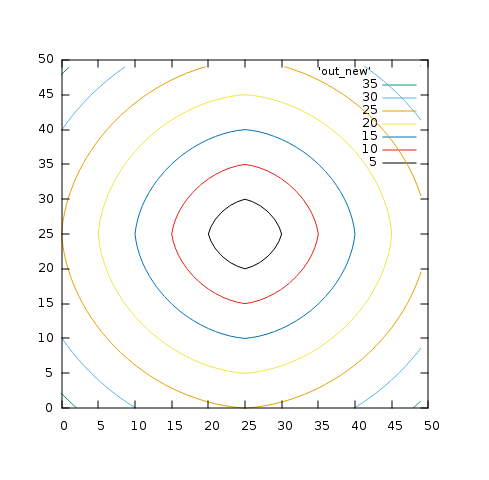
\includegraphics[width=0.7\linewidth]{img/eikonal_simple_surface.png}
  \hfil \caption{Линии уровня эйконала с $F\equiv 1$ }
  \label{fig:eikonal-surface}
\end{figure}

\begin{figure}[H]
  \centering
  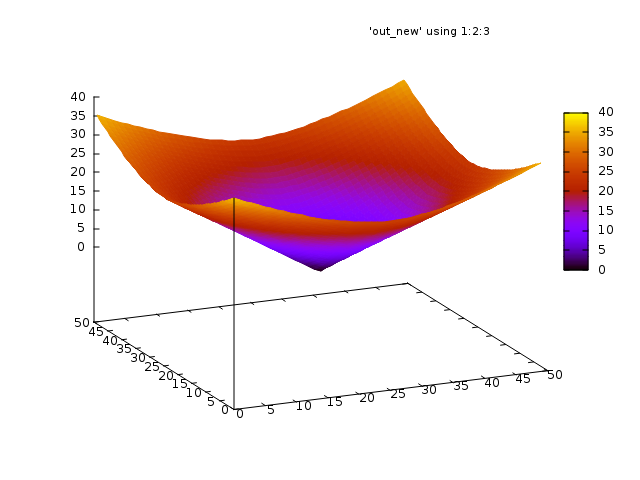
\includegraphics[width=\linewidth]{img/eikonal_simple_3d.png}
  \hfil \caption{Трехмерный график численного решения эйконала с
    $F\equiv 1$}
  \label{fig:eikonal-surface-3d}
\end{figure}

Если мы добавим барьер для распространения волн, т.е. в точках лежащих
на некотором прямоугольнике установим значение $0$. Мы получим
следующий результат. Смотри рисунок~\ref{fig:barier_surface}.

\begin{figure}[H]
  \centering
  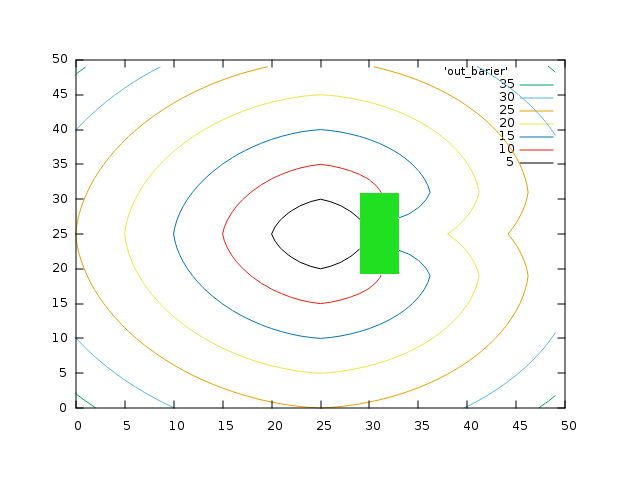
\includegraphics[width=\linewidth]{img/barier_surface.png}
  \hfil \caption{Линии уровня эйконала с $F\equiv 1$, с препятствием}
  \label{fig:barier_surface}
\end{figure}

\subsection{Множество достижимости импульсной системы}
\label{sec:ids}

В работах \cite{AVS2016, AV2015_1,AV2015_2} предлагалось считать множество
достижимости импульсной управляемой системы \cite{D2003}. В использованном в
тех работах методе, были существенные ограничения на систему ограничений на
управление. Для описаний ограничений на управлении использовалась $l_1$
метрика. Методы численных решений уравнений эйконала позволяют нам
использовать евклидову метрику, правда за счет некоторого упрощения
управляемых систем.

Для начала взглянем на обычную управляемую систему, расширение
множества траекторий которой и приводит к импульсной системе. Будем
работать с системой следующего вида. 

\begin{equation}
  \label{system_s}
  \begin{array}{l}
    \dot{x}(t)=E \cdot F(x)v(t), \quad x(0)=x_0, \\[8pt]
    v(t)\geq 0  \qquad \forall\, t\in T = [0,t_1], \qquad
    \displaystyle\int_{0}^{t_1} ||v(t)||dt\leq V.
  \end{array} 
\end{equation}

Здесь
\begin{itemize}
  \item $E$ --- единичная матрица.
  \item $||v||:=\sqrt{v_1^2+v_2^2}$
  \item $x(\cdot)$ --- абсолютно непрерывная вектор-функция
    (траектория), $x(t)\in {\mathbb R}^n,$
  \item $v(\cdot)$ --- измеримая существенно ограниченная
    вектор-функция (управление),
  
  \item $V$ --- заданная величина интегрального ресурса управления
    $v$.
\end{itemize}

Пару функций $\bigl(x(\cdot),v(\cdot)\bigr),$ удовлетворяющих
системе \eqref{system_s}, будем называть процессом системы \eqref{system_s}.

Будем предполагать, что вектор-функция $f$ является функцией из
$L_{\infty}(T,\mathbb{R}^2)$.
     
Множество обычных траекторий системы \eqref{system_s} будет состоять
из функций, имеющих равномерно ограниченные полные вариации на отрезке
$T$. Следовательно, любая последовательность траекторий будет
содержать подпоследовательность, поточечно сходящуюся к некоторой
функции ограниченной вариации. Именно такие функции, являющиеся
поточечными пределами последовательностей обычных траекторий, в
дальнейшем будут называться разрывными (или обобщенными) решениями
системы \eqref{system_s}.

 Рассмотрим систему \eqref{system_d} соответствующую системе
\eqref{system_s}.

\begin{equation}
  \label{system_d}
  \begin{array}{l}
    dx(t)=f\big(t,x(t)\big)dt+G\big(t,x(t)\big)\pi(\mu), \quad
    x(0)=x_0, \\[8pt]
    \pi(\mu) \in \mathcal{W}(T)
  \end{array} 
\end{equation}

Здесь $T=[0,t_1]$ --- заданный отрезок времени, $x(\cdot)$ ---
непрерывная справа на $(0,t_1]$ функция ограниченной вариации, $x(t)
\in \mathbb{R}^2$. Решения системы \eqref{system_d}, соответсвующие
управлению $\pi(\mu)$, понимаются как решения интегрального уравнения
с мерой

\begin{equation*}
  x(t) = x_0  + \int_0^t E\cdot F(t,x(t)) \mu_c(dt) +
  \sum_{s \le t,\\s \in S_d(\mu)} (z_s(d_s) - x(s-)), \quad t \in (0,t_1]
\end{equation*}

где для каждого $s \in S_d(\mu)$ функция $z_s(\cdot)$ --- решение
дифференциального уравнения

\begin{equation*}
  \frac{dz_s(\tau)}{d\tau} = E\cdot f(s,z_s(\tau))\omega_s(\tau), 
	\quad z_s(0)=x(s-)
\end{equation*}

Таким образом, при расширении системы \eqref{system_s} и переходе к
соответствующей импульсной системе \eqref{system_d} мы к обычным
(абсолютно непрерывным) траекториям добавляем все частичные
поточечные пределы последовательностей обычных
траекторий. Полученное множество будем называть множеством
траекторий импульсной системы, соответствующей \eqref{system_s} и будем
обозначать импульсную систему символом \eqref{system_d} Поясним,
что если в системе \eqref{system_d} траектории могут иметь скачки,
то их обобщенные производные будут содержать дельтообразные
составляющие --- импульсы; следовательно, импульсы появятся в
соответствующих управлениях, отсюда и названия импульсной системы и
импульсного управления.


Функция ограниченной вариации $x(\cdot)$ называется траекторией импульсной
системы \eqref{system_d} (или обобщенным (разрывным) решением системы
\eqref{system_s}), если найдется такая последовательность траекторий системы
\eqref{system_s} $\bigl\{x_k(\cdot)\bigr\}$, что выполняется условие 

\begin{equation*}
  x_k(t)\to x(t) \quad  \forall \, t\in [0,T].
\end{equation*}

Определим \emph{множество достижимости} в момент  времени $t=t_1$
импульсной системы \eqref{system_d}. Обозначим это множество через 
$ {\mathcal R}_V(t_1)$. Это множество из  пространства ${\mathbb R}^n$
(конечномерное  множество), оно состоит из точек $x_b,$ в  которые в
момент $t=t_1$ попадают траектории  системы \eqref{system_d}, выходящие
в начальный  момент из начальной точки $x_0$.

Возьмем пример динамической системы:

\begin{equation*}
  \begin{aligned}[b]
    &\dot{x_1}(t) = (1/((x_1(t)+0.1) * (x_2(t)+0.1))v_1(t), & x_1(0)=50\\
    &\dot{x_2}(t) = (1/((x_1(t)+0.1) * (x_2(t)+0.1))v_2(t), & x_2(0) = 50\\[8pt]
    &v_1(t) \ge 0, v_2(t) \ge 0 \\
    &\int_{0}^{1} \sqrt{(v_1(t)^2) + (v_2(t))^2} dt \le V
  \end{aligned}
\end{equation*}

Множеством достижимости для конкретного $V$ здесь будут все значения
решения, которые меньше или равны заданному $V$. Численные методы
решения эйконала порождают интегральную воронку: все возможные
множества достижимости для значения $V \in [0,V_{max}]$

На рисунке~\ref{fig:impulse-example-levels} представлено такая
интегральная воронка через линии уровня.

\begin{figure}[H]
  \centering
  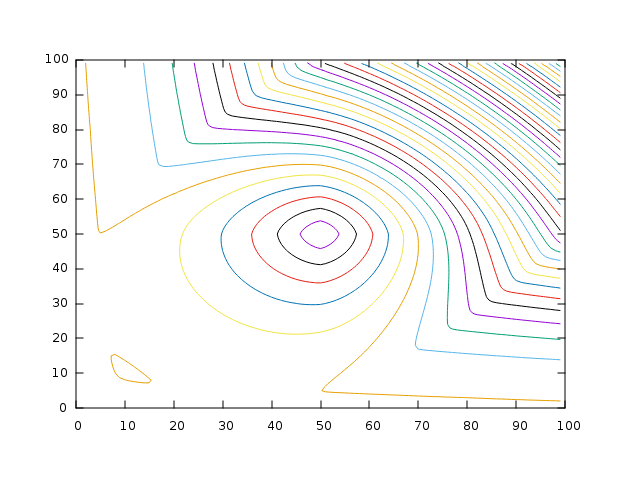
\includegraphics[width=0.5\linewidth]{img/impulse-example-levels.png}
  \hfil \caption{Линии уровня множества достижимости}
  \label{fig:impulse-example-levels}
\end{figure}

В виде трехмерной поверхности график можно увидеть на
рисунке~\ref{fig:impulse-example}

\begin{figure}[H]
  \centering
  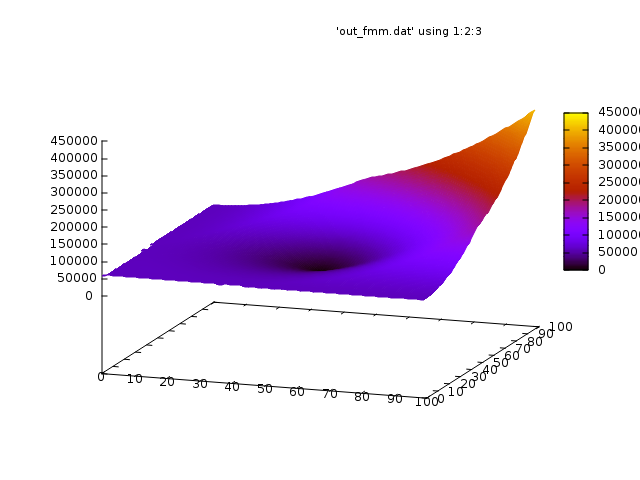
\includegraphics[width=\linewidth]{img/impulse-example.png}
  \hfil \caption{Интегральная воронка в трехмерном виде}
  \label{fig:impulse-example}
\end{figure}


\subsection{Shape from shading}
\label{sec:shape-from-shading}

Еще одним важным приложением численных алгоритмов решения уравнения
эйконала является задача восстановления по черно-белой картинке (или
фотографии) форму исходного объекта \cite{SFS2009,JDM2008}. Это понятие также
не переводится в русскоязычных публикациях.  Дословно это понятие
значит построение поверхности от тени. На изображении, лишенном цвета,
нашему глазу предоставляется информация о яркости соответствующей
точки. Наш глаз может благодаря ей строить форму объекта.  

Яркость изображения пропорциональна излучению от поверхности к
наблюдателю

\begin{equation}
  \label{eq:sfs:1}
  E_i=\mu L_s,
\end{equation}

где параметр $\mu$ зависит от параметров камеры (таких как диаметр
линзы, фокальное расстояние и т.д.).
Мы полагаем, что источник освещения один и находится примерно там же,
где и глаз наблюдателя. Кроме того отсутствуют отражения. Яркость
изображения пропорциональна излучению поверхности, изображенной на
нем. В этом случае отношение между излучением точки поверхности с
нормалью в этой точке и направлением к источнику света описывается 
Двулучевой функцией отражательной способности (ДФОС), которая является
константой для Ламбертиановской поверхности.

\begin{equation}
  \label{eq:sfs:4}
  L_s=\frac{\alpha}{\pi}E_s,
\end{equation}

где $\alpha$ --- альбедо, а $E_s$ --- интенсивностью
излучения. Наконец, интенсивность излучения $E_s$ определяется как:

\begin{equation}
  \label{eq:sfs:5}
  E_s = I_0\frac{cos(\theta_i)}{r^2},
\end{equation}

где $I_0$ это интенсивность источника света, $r$ --- расстояние между
источником света и точкой поверхности и $theta_i$ --- угол между
нормалью к точке поверхности и направлением на источник света.

Из \eqref{eq:sfs:1}, \eqref{eq:sfs:4} и \eqref{eq:sfs:5} получим яркость
изображения:

\begin{equation}
  \label{eq:sfs:6}
  E_i = \sigma\frac{cos(\theta_i)}{r^2},
\end{equation}

где $\sigma$ это постоянный коэффициент, связанный с параметрами
системы формирования изображения, интенсивности источника света и
альбедо поверхности.

Мы можем получит формулы для того, чтобы преобразовать яркость в
коэффициент, пропорциональный углу наклона нашей поверхности.  На
языке python был написан скрипт (листинг 8), который переводит
информацию по яркости изображения в такой параметр, т.е. чем выше
яркость, тем меньше в этой точке наклон поверхности относительно
ортогонального к нам. Тем самым мы получаем $F$ для уравнения
эйконала, по которой ищем решение. Оно и будет той самой поверхностью,
которую нам нужно достать из фотографии

\vspace{1em} Листинг 8 --- Скрипт преобразования изображение в $F$ для
уравнения эйконала \normalsize
\begin{verbatim}
#!/usr/bin/env python

from PIL import Image
import scipy as sc
import sys
import math

def main():
    im = Image.open(sys.argv[1])
    print im.height* im.width, 3
    data = sc.asarray(im.convert("L"))

    out = sc.empty([im.height, im.width])

    max_out = 0
    
    max_val = data.max()
    lst = []
    for i in range(len(data)):
        for j in range(len(data[i])):
            if abs(data[i][j]) > 0.01:
                tst = math.sqrt(
          (1.0*max_val/data[i][j])**2 - 1)
                if abs(tst) > 0.1:
                    out[i][j] = 1.0/tst
                else:
                    out[i][j]= sc.inf
            else:
                out[i][j]= 0
            if out[i][j]>max_out:
                max_out = out[i][j]

    for i in range(len(data)):
        for j in range(len(data[i])):
            if data[i][j]==max_val:
                print i,j,out[i][j],0
            else:
                print i,j,out[i][j],sc.inf

if __name__ == '__main__':
    main()
\end{verbatim}
\large

Далее приведем несколько примеров картинок и трехмерных поверхностей,
полученных на них. Сперва было построено тестовое синтетическое
изображение сферы для тестирования алгоритма: рисунки~\ref{fig:ex:1:in} 
и ~\ref{fig:ex:1:out}

\begin{figure}[H]
  \centering
  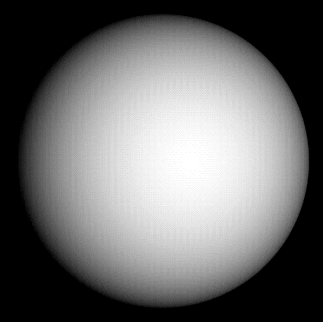
\includegraphics[width=0.5\linewidth]{img/sphere_in.png}
  \hfil \caption{Сфера исходное изображение}
  \label{fig:ex:1:in}
\end{figure}

\begin{figure}[H]
  \centering
  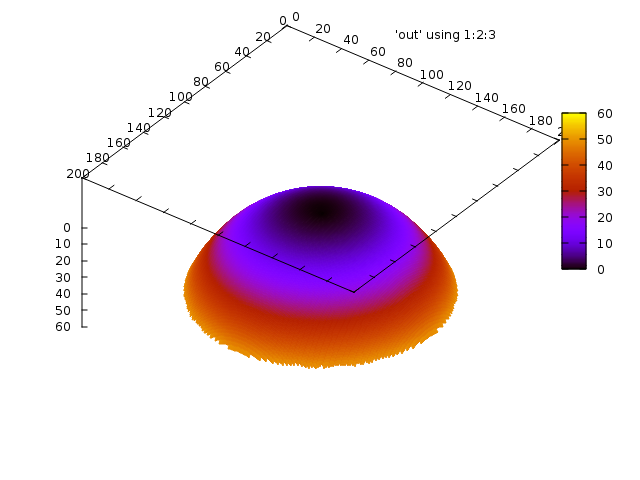
\includegraphics[width=0.5\linewidth]{img/sphere.png}
  \hfil \caption{Трехмерная поверхность сферы по фотографии}
  \label{fig:ex:1:out}
\end{figure}

Затем было решено попробовать несколько стандартных фигур, в работах
по компьютерному зрению и 3D моделированию: чайник
(рисунки~\ref{fig:ex:2:in} и ~\ref{fig:ex:2:out}) и маска Моцарта
(рисунки~\ref{fig:ex:3:in} и ~\ref{fig:ex:3:out}).

\begin{figure}[H]
  \centering
  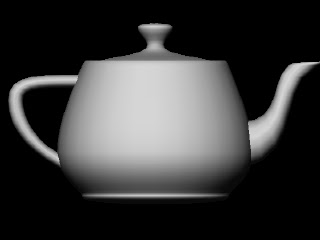
\includegraphics[width=0.5\linewidth]{img/teapot_in.jpg}
  \hfil \caption{Чайник исходное изображение}
  \label{fig:ex:2:in}
\end{figure}

\begin{figure}[H]
  \centering
  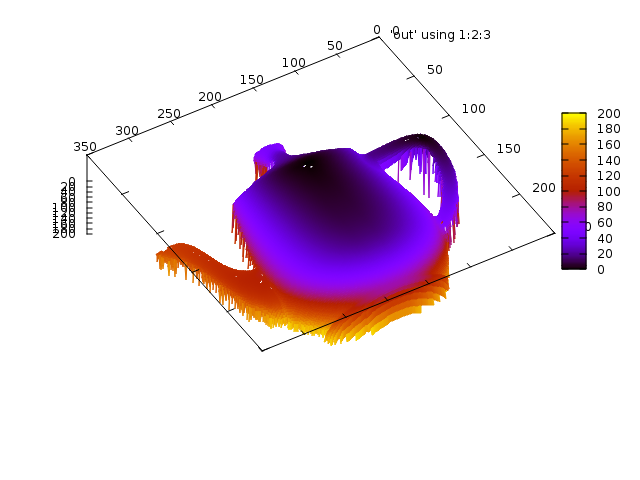
\includegraphics[width=0.5\linewidth]{img/teapot.png}
  \hfil \caption{Трехмерная поверхность чайника по фотографии}
  \label{fig:ex:2:out}
\end{figure}

\begin{figure}[H]
  \centering
  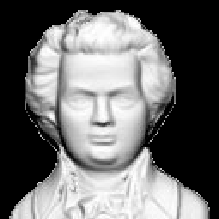
\includegraphics[width=0.5\linewidth]{img/mozart_in.png}
  \hfil \caption{Моцарт исходное изображение}
  \label{fig:ex:3:in}
\end{figure}

\begin{figure}[H]
  \centering
  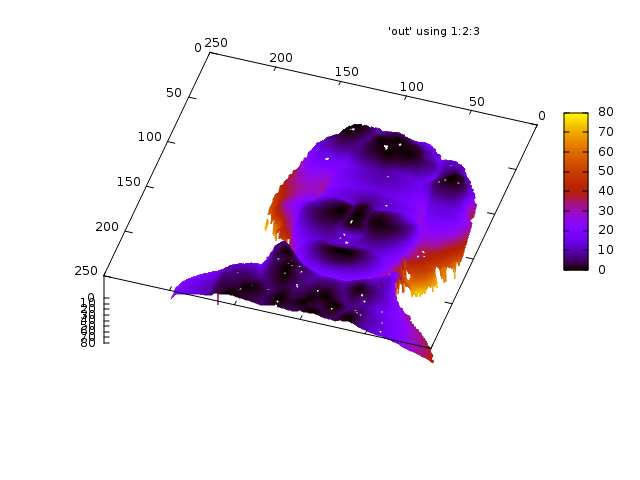
\includegraphics[width=0.5\linewidth]{img/mozart.png}
  \hfil \caption{Трехмерная поверхность Моцарта по фотографии}
  \label{fig:ex:3:out}
\end{figure}

После проверена работоспособность на фотографиях. Поскольку модель
распространения света у нас весьма упрощенная и может адекватно
обрабатывать только идеально матовые поверхности здесь результат
несколько менее точен: рисунки~\ref{fig:ex:4:in}, ~\ref{fig:ex:4:out1}
и~\ref{fig:ex:4:out2})

\begin{figure}[H]
  \centering
  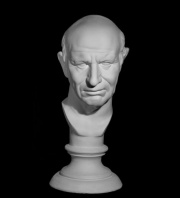
\includegraphics[width=0.5\linewidth]{img/man_in.jpg}
  \hfil \caption{исходная фотография}
  \label{fig:ex:4:in}
\end{figure}

\begin{figure}[H]
  \centering
  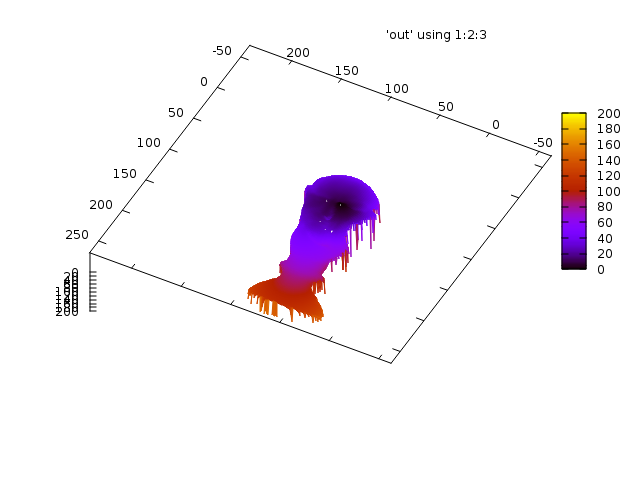
\includegraphics[width=0.5\linewidth]{img/man_all.png}
  \hfil \caption{Трехмерная поверхность по фотографии общая}
  \label{fig:ex:4:out1}
\end{figure}

\begin{figure}[H]
  \centering
  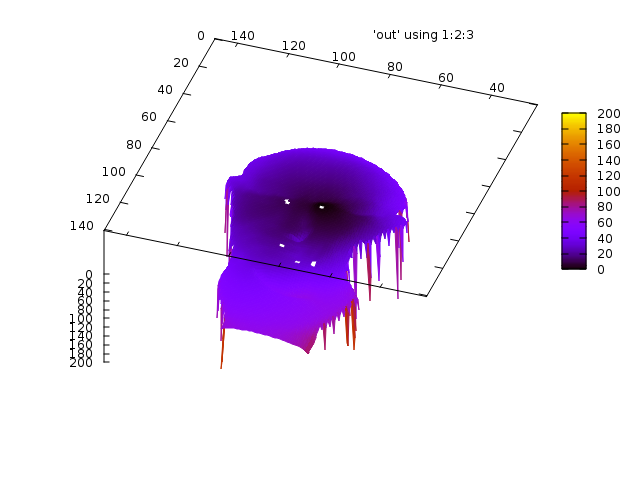
\includegraphics[width=0.5\linewidth]{img/man_detail.png}
  \hfil \caption{Детали трехмерной поверхности по фотографии }
  \label{fig:ex:4:out2}
\end{figure}


\pagebreak
\section*{Заключение}
\addcontentsline{toc}{section}{Заключение}
\label{sec:conclusion}

В работе были представлены реализации численных методов решения
уравнения эйконала. Наиболее важным результатом является вариант
алгоритма FMM, предназначенный для аппроксимации множеств достижимости
импульсных управляемых систем. Рассмотрен ряд примеров, включая
вычисление расстояний на плоскости при неоднородной метрике и
восстановление формы изображения по черно-белому снимку. Разработаны
реализации на языке C. Проведены численные эксперименты с параллельным
вариантом FSM.

В задаче аппроксимации множеств достижимости разработанные программы
показывают себя с лучшей стороны, помогают в поисках аналитического
решения и позволяют создавать иллюстрации. В задаче восстановления
формы тела для синтезированных изображений задача решается с высокой
точностью; к сожалению, не удалось протестировать алгоритм в реальных
условиях. С учетом небольшого времени работы для актуальных постановок
задач использовать параллельную реализацию, как правило,
нецелесообразно; это потребуется, например, для аппроксимации множеств
достижимости систем в размерности 3 (в задаче 1) или при обработке
снимков высокого разрежения (в задаче 2). Изучение масштабируемости
параллельных реализаций представляет собой одно из возможных
направлений дальнейшей работы.
\pagebreak
\begin{thebibliography}{99}
  \addcontentsline{toc}{section}{Список литературы}


\bibitem{KL2011}Казаков А. Л., Лемперт А. А. Об одном подходе к
  решению задач оптимизации, возникающих в транспортной логистике
  //Автоматика и телемеханика. – 2011. – №. 7. – С. 50-57.

\bibitem{KLN2016}Казаков А. Л., Лемперт А. А., Нгуен Г. Л. Об одном
  алгоритме построения упаковки конгруэнтных кругов в неодносвязное
  множество с неевклидовой метрикой //Вычислительные методы и
  программирование. – 2016. – Т. 17. – №. 2. – С. 177-188.

\bibitem{G1956}Годунов С. К. Разностный метод численного расчета
  разрывных решений уравнений гидродинамики //Математический
  сборник. – 1959. – Т. 47. – №. 3. – С. 271-306.
  
\bibitem{D2003}Дыхта В. А., Самсонюк О. Н. Оптимальное импульсное
  управление с приложениями. – М. : Физматлит, 2003.

\bibitem{V2005} Вдовина О. И., Сесекин А. Н. Численное построение
  областей достижимости для систем с импульсным управлением //Труды
  Института математики и механики УрО РАН. – 2005. – Т. 11. – №. 1. –
  С. 65-73.

\bibitem{L2016} Лебедев П. Д., Успенский А. А. Построение функции
  оптимального результата и рассеивающих линий в задачах
  быстродействия с невыпуклым целевым множеством //Труды Института
  математики и механики УрО РАН. – 2016. – Т. 22. – №. 2. –
  С. 188-198.

  
\bibitem{P2008} Лебедев П. Д., Успенский А. А., Ушаков
  В. Н. Построение минимаксного решения уравнения типа эйконала
  //Труды Института математики и механики УрО РАН. – 2008. – Т. 14. –
  №. 2. – С. 182-191.
  
\bibitem{E2014}Москаленский Е. Д. О нахождении точных решений
  двумерного уравнения эйконала для случая, когда фронт волны,
  распространяющейся в среде, является окружностью //Сибирский журнал
  вычислительной математики. – 2014. – Т. 17. – №. 4. – С. 363-372.

\bibitem{B2006} Боровских А. В. Группы эквивалентности уравнений
  эйконала и классы эквивалентных уравнений //Новосибирский
  государственный университет. – Новосибирский государственный
  университет, 2006.

\bibitem{B2014} Боровских А. В. Уравнение эйконала для анизотропной
  среды //Труды семинара имени ИГ Петровского. – 2013. – Т. 29. –
  №. 0. – С. 162-229.

\bibitem{I2005} Иванов Д. И., Иванов И. Э., Крюков И. А. Алгоритмы
  приближенного решения некоторых задач прикладной геометрии,
  основанные на уравнении типа Гамильтона–Якоби //Журнал
  вычислительной математики и математической физики. – 2005. –
  Т. 45. – №. 8. – С. 1345-1358.

\bibitem{N2015} Дучков А. А. и др. Параллельный алгоритм решения
  уравнения эйконала для трехмерных задач сейсморазведки
  //Новосибирский государственный университет. – Новосибирский
  государственный университет, 2015.
  
\bibitem{AVS2016} Апанович Д. В., Воронов В. А., Самсонюк
  О. Н. Построение множества достижимости двумерной импульсной
  управляемой системы с билинейной структурой //Известия Иркутского
  государственного университета. Серия: Математика. – 2016. – Т. 15.

\bibitem{AV2015_1} Апанович Д. В., Воронов В. А. Численная аппроксимация
  множеств достижимости нелинейных импульсных управляемых систем. //
  Теория управления и математическое моделирование: Тезисы докладов
  Всероссийской конференции с международным участием, посвященной
  памяти профессора Н. В. Азбелева и профессора Е. Л. Тонкова (Ижевск,
  Россия, 9–11 июня 2015 г.). Ижевск: Изд-во «Удмуртский университет»,
  2015. С. 24-25.

\bibitem{AV2015_2} Апанович Д. В., Воронов В. А. Численная
  аппроксимация неодносвязного множества достижимости нелинейной
  импульсной управляемой системы. // Тезисы докладов III
  Российско-монгольской конференции молодых ученых по математическому
  моделированию, вычислительно-информационным технологиям и управлению
  (Иркутск (Россия) – Ханх (Монголия), 23 июня – 30 июня 2015 г.). –
  Иркутск: Научно-организационный отдел ИДСТУ СО РАН, 2015. С. 17.
  
\bibitem{S1999} Sethian J. A. Level set methods and fast marching
  methods: evolving interfaces in computational geometry, fluid
  mechanics, computer vision, and materials science. – Cambridge
  university press, 1999. – Т. 3.

\bibitem{B2006}Berczynski P. et al. Diffraction of a Gaussian beam in
  a three-dimensional smoothly inhomogeneous medium: an eikonal-based
  complex geometrical-optics approach //JOSA A. – 2006. – Т. 23. –
  №. 6. – С. 1442-1451.

\bibitem{W1969} Walther A. Lenses, wave optics, and eikonal functions
  //JOSA. – 1969. – Т. 59. – №. 10. – С. 1325-1331.
  
\bibitem{AV2003} Sethian J. A., Vladimirsky A. Ordered upwind methods
  for static Hamilton--Jacobi equations: Theory and algorithms //SIAM
  Journal on Numerical Analysis. – 2003. – Т. 41. – №. 1. –
  С. 325-363.
  
\bibitem{V1983} Crandall M. G., Lions P. L. Viscosity solutions of
  Hamilton-Jacobi equations //Transactions of the American
  Mathematical Society. – 1983. – Т. 277. – №. 1. – С. 1-42.

\bibitem {V1984} Crandall M. G., Evans L. C., Lions P. L. Some
  properties of viscosity solutions of Hamilton-Jacobi equations
  //Transactions of the American Mathematical Society. – 1984. –
  Т. 282. – №. 2. – С. 487-502.

  
\bibitem{F2005} Zhao H. K. A fast sweeping method for eikonal
  equations //Mathematics of computation. – 2005. – Т. 74. – №. 250. –
  С. 603-627.

\bibitem{K2017} Кормен Т. и др. Алгоритмы. Построение и анализ:[пер. с
  англ.]. – Издательский дом Вильямс, 2017.

\bibitem{R1974} Porter T., Simon I. Random insertion into a priority
  queue structure //IEEE Transactions on Software Engineering. –
  1975. – №. 3. – С. 292-298.


\bibitem{F1987} Fredman M. L., Tarjan R. E. Fibonacci heaps and their
  uses in improved network optimization algorithms //Journal of the
  ACM (JACM). – 1987. – Т. 34. – №. 3. – С. 596-615.

  
\bibitem{J2015}Gómez González J. V. Fast Marching Methods in path and
  motion planning: improvements and high-level applications. – 2015.
  
\bibitem{C2013}Capozzoli A. et al. A comparison of Fast Marching, Fast
  Sweeping and Fast Iterative Methods for the solution of the eikonal
  equation //Telecommunications Forum (TELFOR), 2013 21st. – IEEE,
  2013. – С. 685-688.
  
\bibitem{KOT2005} Kao C. Y., Osher S., Tsai Y. H. Fast Sweeping
  Methods for Static Hamilton--Jacobi Equations //SIAM journal on
  numerical analysis. – 2005. – Т. 42. – №. 6. – С. 2612-2632.

\bibitem{A2006}Alvarez O. et al. Convergence of a first order scheme
  for a non-local eikonal equation //Applied numerical mathematics. –
  2006. – Т. 56. – №. 9. – С. 1136-1146.
  
\bibitem{FSA2007}Qian J., Zhang Y. T., Zhao H. K. A fast sweeping
  method for static convex Hamilton–Jacobi equations //Journal of
  Scientific Computing. – 2007. – Т. 31. – №. 1. – С. 237-271.
  
\bibitem{FS2007} Qian J., Zhang Y. T., Zhao H. K. Fast sweeping
  methods for Eikonal equations on triangular meshes //SIAM Journal on
  Numerical Analysis. – 2007. – Т. 45. – №. 1. – С. 83-107.

\bibitem{C2017} Клеменс Б. Язык С в XXI веке. – Litres, 2017.

\bibitem{N1989}Seiler M. C., Seiler F. A. Numerical recipes in C: the
  art of scientific computing //Risk Analysis. – 1989. – Т. 9. –
  №. 3. – С. 415-416.
  
\bibitem{AP2016} Реймонд Э. C. Искусство программирования для Unix. –
  Издательский дом Вильямс, 2005.

\bibitem{F2002} LeVeque R. J. Finite volume methods for hyperbolic
  problems. – Cambridge university press, 2002. – Т. 31.

\bibitem{T2002} {А. В. Скворцов} Триангуляция Делоне и её применение. –
  Томск: Изд-во Том. ун-та, 2002.

\bibitem{SFS2009} Prados E., Faugeras O. Shape from shading: a
  well-posed problem? //Computer Vision and Pattern Recognition,
  2005. CVPR 2005. IEEE Computer Society Conference on. – IEEE,
  2005. – Т. 2. – С. 870-877.
  
\bibitem{JDM2008}Durou J. D., Falcone M., Sagona M. Numerical methods
  for shape-from-shading: A new survey with benchmarks //Computer
  Vision and Image Understanding. – 2008. – Т. 109. – №. 1. –
  С. 22-43.
\end{thebibliography}

\pagebreak
\section*{Приложение А}
\addcontentsline{toc}{section}{Приложение А}
\label{sec:appl}

\vspace{1em}
Листинг А.1 --- Текст программы для решения уравнения эйконала FMM

\small
\begin{verbatim}

// -*- compile-command: "cc `pkg-config
 --libs --cflags glib-2.0 gsl` -lm solver.c " -*-

#include <stdio.h>
#include <math.h>
#include <glib.h>
#include <gsl/gsl_matrix.h>
#include <gsl/gsl_poly.h>

const double lbound_x = -8.0;
const double rbound_x = 8.0;
const double lbound_y = -8.0;
const double rbound_y = 8.0;

const double h      = 0.05;
const double x_step = 0.05;
const double y_step = 0.05;


gsl_matrix* T;
gsl_matrix* K;
GQueue* active_nodes;

typedef struct {
  int dim_1, dim_2;
  double *data;
} Grid;

typedef struct {
  int i,j;
} Node;

Node* make_node(int i, int j);
void node2point(Node node, 
      double* x, double *y);
void prt(gpointer item);
gint cmp(gconstpointer a, 
   gconstpointer b, gpointer _);

double g(Node node);
double speed(Node node);
gboolean is_internal(Node node);
/* get_neighbours(Node* node, GList nbours); */
void init();
void process_neighbour(int i, int j);


int main(void)
{
  int dim_1 = (rbound_x - lbound_x) / x_step;
  int dim_2 = (rbound_y - lbound_y) / y_step;
  T = gsl_matrix_alloc(dim_1, dim_2);
  K = gsl_matrix_calloc(dim_1, dim_2);

  /* printf("%d %d\n", dim_1, dim_2); */
  active_nodes = g_queue_new();

  init();

  while (!g_queue_is_empty(active_nodes)) {
    Node* node = g_queue_pop_head(active_nodes);
    gsl_matrix_set(K, node->i, node->j,0);
    process_neighbour(node->i - 1, node->j);
    process_neighbour(node->i + 1, node->j);
    process_neighbour(node->i, node->j - 1);
    process_neighbour(node->i, node->j + 1);
  }

  int i, j;
  for (i = 0; i < T->size1; ++i) {
    for (j = 0; j < T->size2; ++j){
      double val = gsl_matrix_get(T, i, j);
      printf("% lf % lf % lf\n", i*h, j*h, val);
    }
    putchar('\n');
  }
  return 0;
}

void process_neighbour(int i, int j)
{
  Node node = {i,j};
  if (!is_internal(node) || 
   !gsl_matrix_get(K, i, j)) return;
  double lT = gsl_matrix_get(T, i - 1, j);
  double rT = gsl_matrix_get(T, i + 1, j);
  double uT = gsl_matrix_get(T, i, j - 1);
  double dT = gsl_matrix_get(T, i, j + 1);

  double mini = lT < rT ? lT : rT;
  double minj = uT < dT ? uT : rT;

  double time;

  if (finite(mini) && isinf(minj))
    time = mini + x_step/speed(node);
  else if (finite(minj) && isinf(mini))
    time = minj + y_step/speed(node);
  else if (finite(mini) && finite(minj)){
    double a = 1/(x_step*x_step) + 
               1/(y_step*y_step);
    double b = -2 * (mini/pow(x_step, 2) +
                      minj/pow(y_step,2));
    double c = pow(mini/x_step, 2) + 
             pow(minj/y_step, 2) - 
               1.0/speed(node);
    double x1,x2;
    int croots = gsl_poly_solve_quadratic(a,b,c, &x1, &x2);
    if (croots == 0)
      time = INFINITY;
    else if (croots == 1)
      time = x1;
    else if (croots == 2)
      time = x2;
  }
  if (time < gsl_matrix_get(T, i, j)){
    gsl_matrix_set(T, i, j, time);
    g_queue_insert_sorted(active_nodes,
                          make_node(i,j),
                          (GCompareDataFunc)cmp,NULL);
  }
}

Node* make_node(int i, int j)
{
  Node* node = g_new(Node,1);
  node->i = i;
  node->j = j;
  return node;
}

void prt(gpointer item)
{
  int i = ((Node*)item)->i;
  int j = ((Node*)item)->j;
  printf("[%d,%d] = %g\n",i,j,gsl_matrix_get(T,i,j));
}

gint cmp(gconstpointer a, gconstpointer b, gpointer _)
{
  int i = ((Node*)a)->i;
  int j = ((Node*)a)->j;
  double val1 = gsl_matrix_get(T,i,j);
  i = ((Node*)b)->i;
  j = ((Node*)b)->j;
  double val2 = gsl_matrix_get(T,i,j);

  return floor(val1 - val2);
}

void node2point(Node node, double* x, double *y)
{
  *x = lbound_x + x_step * node.i;
  *y = lbound_y + y_step * node.j;
  return;
}

double g(Node node)
{
  double x, y;
  node2point(node, &x, &y);
  return x*x + y*y - 0.0001;
}

double speed(Node node)
{
  double x, y;
  node2point(node, &x, &y);
  double circle = pow(x,2) + pow(y - 3, 2) - 4;
  return 1 + 1.0/(pow(circle, 2) + 0.1);
}

gboolean is_internal(Node node) {
  int i = node.i;
  int j = node.j;
  return i > 0 && i < T->size1 - 1 && 
     j > 0 && j < T->size2 - 1;
}

void process_node(int i, int j)
{
  Node n1 = {.i = i, .j=j};
  if (g(n1) <= 0){
    gsl_matrix_set(T,i,j,0);
    gsl_matrix_set(K,i,j,1);
    if (is_internal(n1))
      g_queue_push_head(active_nodes,
                        make_node(i, j));
  } else {
    gsl_matrix_set(T,i,j,INFINITY);
    gsl_matrix_set(K,i,j,1);
  }

}
void init()
{
  int i, j;
  for (i = 0; i < T->size1; ++i)
    for(j = 0; j < T->size2; ++j)
      process_node(i, j);
}
\end{verbatim}
\large

\vspace{1em}
Листинг А.2 --- Текст программы для решение уравнения эйконала FSM
\small
\begin{verbatim}
// -*- compile-command: "cc -o sfs-fsm `pkg-config --libs
    --cflags glib-2.0 gsl` -lm sfs-fsm.c " -*-

#include <stdio.h>
#include <math.h>
#include <glib.h>
#include <unistd.h>
#include <stdbool.h>
#include <gsl/gsl_matrix.h>
#include <gsl/gsl_poly.h>

const int dim = 2;
double h = 1;

gsl_matrix* T;
gsl_matrix* F;

int sweep_dirs[2];

gboolean is_debug = 0;

void init();
double process_neighbour(int i, int j);

void get_sweep_dirs(/* int* sweep_dirs */);
bool sweep();

int main(int argc, char **argv)
{
  int dim_1,dim_2;
  int i, j;
  int opt;
  while ((opt = getopt(argc, argv, "d")) != -1) {
    switch (opt) {
    case 'd':
      is_debug = 1;
      puts("DEBUG:::OUTPUT\n");
      break;
    default: /* '?' */
      fprintf(stderr, "Usage: %s [-d]\n",
              argv[0]);
      exit(EXIT_FAILURE);
    }
  }

  /* puts("set grid\nset hidden3d\n" */
  /*      "$mapl << EOD"); */

  if (is_debug) puts("READ image size\n");
  scanf("%d%d", &dim_1, &dim_2);

  T = gsl_matrix_alloc(dim_1, dim_2);
  F = gsl_matrix_alloc(dim_1,dim_2);
  active_nodes = g_queue_new();
  init();

  bool stop = false;
  int sweep_count = 0;
  int pos[dim];
  for(int k = 1; k <=4; k++){
    get_sweep_dirs(sweep_dirs);
    /* stop = sweep(dim - 1,pos); */
    int _i, _j;
    for (int i = 0; i < F->size1; i++){
      for (int j = 0; j < F->size2; j++) {
        if (sweep_dirs[0] == 1)
          _i = i;
        else
          _i = F->size1 - i - 1;
        if (sweep_dirs[1] == 1)
          _j = j;
        else
          _j = F->size2 - j - 1;
        double time = process_neighbour(_i,_j);

        if (time < gsl_matrix_get(T, _i, _j)){
               
          gsl_matrix_set(T, _i, _j, time);
          /* stop = false; */
        } 

      }
    }
  }
  for (i = 0; i < T->size1; ++i) {
    for (j = 0; j < T->size2; ++j){
      double val = gsl_matrix_get(T, i, j);
      printf("%f %f %f\n", i*h,j*h,val);
    }
    putchar('\n');
  }

  /* puts("EOD\n" */
  /*      "splot '$mapl' matrix with lines notitle"); */
        
  return 0;
}

double process_neighbour(int i, int j)
{
  Node node = {i,j};
  /* if (!gsl_matrix_get(K, i, j)) return; */
  if (is_debug)
    printf("neighbour - [%d %d]\n", i, j );

  double lT = i > 0 ? 
    gsl_matrix_get(T, i - 1, j): 
   INFINITY;
  double rT = i < T->size1 - 1 ? 
   gsl_matrix_get(T, i + 1, j): 
   INFINITY;
  double uT = j > 0 ? 
   gsl_matrix_get(T, i, j - 1): 
   INFINITY;
  double dT = j < T->size2 - 1 ? 
   gsl_matrix_get(T, i, j + 1): 
   INFINITY;


  double mini = lT < rT ? lT : rT;
  double minj = uT < dT ? uT : dT;
  if (is_debug)
    printf("\t%g %g %g %g => %g %g\n", 
       lT, rT, uT, dT, mini, minj);

  double time = INFINITY;
  if (is_debug)
    printf("\tF[%d][%d] = %g\n", i,j,gsl_matrix_get(F, i, j));
  if (finite(mini) && isinf(minj)) {
    if (is_debug){
      printf("\t\tbranch->mini\n");
      printf("\t[%d %d]\n",i,j);
      printf("\t%g %g %g %g => %g %g\n",
          lT, rT, uT, dT, mini, minj);
    }
    time = mini + h/gsl_matrix_get(F, i, j);

  }
  else if (finite(minj) && isinf(mini)) {
    if (is_debug){
      printf("\t\tbranch->minj\n");
      printf("\t[%d %d]\n",i,j);
      printf(
       "\t%g %g %g %g => %g %g\n",
        lT, rT, uT, dT, mini, minj);
    }
    time = minj + h/gsl_matrix_get(F, i, j);


  }
  else if (finite(mini) && finite(minj)){
    if (is_debug)
      printf("\t\tbranch->both\n");
    double idx = 1.0/gsl_matrix_get(F, i, j);
    double a = 2;
    double b = -2 * (mini + minj); 
    double c = pow(mini, 2) + 
       pow(minj, 2) - 
       pow(h/gsl_matrix_get(F, i, j),2);
    double x1=NAN,x2=NAN;
    int croots = 
      gsl_poly_solve_quadratic(a,b,c, &x1, &x2);
    if (is_debug)
      printf(
       "\t%g %g %g = 0: %d roots: x1=%f x2=%f\n"
        ,a,b,c,croots, x1,x2 );
    if (croots == 0)
      time = INFINITY;
    else if (croots == 1)
      time = x1;
    else if (croots == 2)
      time = x2;
  }
  if (is_debug)
    printf("\ttime = %g \n",time );
  return time;
}

Node* make_node(int i, int j)
{
  Node* node = g_new(Node,1);
  node->i = i;
  node->j = j;
  return node;
}

void prt(gpointer item)
{
  int i = ((Node*)item)->i;
  int j = ((Node*)item)->j;
  printf("[%d,%d] = %g\n",
    i,j,gsl_matrix_get(T,i,j));
}

gint cmp(gconstpointer a, 
     gconstpointer b, gpointer _)
{
  int i = ((Node*)a)->i;
  int j = ((Node*)a)->j;
  double val1 = gsl_matrix_get(T,i,j);
  i = ((Node*)b)->i;
  j = ((Node*)b)->j;
  double val2 = gsl_matrix_get(T,i,j);

  return floor(val1 - val2);
}


gboolean is_internal(Node node) {
  int i = node.i;
  int j = node.j;
  return i > 0 && i < T->size1 - 1 
    && j > 0 && j < T->size2 - 1;
}


bool sweep(int n, int* pos)
{
  bool stop = true;
  if (n > 0){
    for (int i = 0; i < F->size2; i++){
      if (sweep_dirs[n] == 1)
        pos[n] = i;
      else
        pos[n] = F->size2 - i - 1;
      stop = sweep(n - 1, pos);
    }
  }
  else
    for (int i = 0; i < F->size1; i++){
      if (sweep_dirs[n] == 1)
        pos[n] = i;
      else
        pos[n] = F->size1 - i - 1;

      double time = 
       process_neighbour(pos[0],pos[1]);

      if (time < gsl_matrix_get(T, pos[0], pos[1])){
               
        gsl_matrix_set(T, pos[0], pos[1], time);
        stop = false;
      } 

    }
  return stop;

}

void get_sweep_dirs(/* int* sweep_dirs */)
{
  for(int i = 0; i < 2; i++) {
    sweep_dirs[i] += 2;
    if (sweep_dirs[i] <= 1)
      break;
    else
      sweep_dirs[i] = -1;
  }
}

void init()
{
  int i, j;
  for (i = 0; i < F->size1; ++i)
    for(j = 0; j < F->size2; ++j) {
      double buf;
      scanf("%lf",&buf);
      gsl_matrix_set(F,i,j,buf);
      gsl_matrix_set(T,i,j,INFINITY);
      /* gsl_matrix_set(K,i,j,1); */
    }

  sweep_dirs[0] = 1;
  sweep_dirs[1] = 1;
        
  long  points_count = 0, point_line = 0;
  scanf("%ld", &points_count);
  int start_i,start_j;

  for (point_line = 0; 
        point_line < points_count; 
          ++point_line) {
    scanf("%d %d",&start_i, &start_j);
    gsl_matrix_set(T,start_i,start_j,0);

  }

}
\end{verbatim}

\end{document}
